\section{A mathematical treatment of worlds and their transformations}\label{sec:A mathematical treatment of worlds and their transformations}

\newthought{We want our} framework to be as general as possible, so we consider worlds as consisting a set of world states, which are distinguishable in some way\footnote{We are building up to using our framework to consider the transformation structure of the world from the perspective of an agent. So when we say \emph{distinguishable in some way} we mean that there is some way for our agent to distinguish between the states.}, and a set of transformations between those world states; these transformation describe how the current state of the world can be changed to other states (\textit{i.e.} the \emph{dynamics of the world}).

We will also make a few simplifications to the worlds we consider:
\paragraph{Deterministic worlds.}
In a deterministic world, every change in the current world state has a single guaranteed effect.
A world that is not deterministic is called \emph{stochastic}; in a stochastic world, the same change to the current world state could produce different results.
We will initially consider deterministic worlds.

\paragraph{Fully observable worlds.}
If complete knowledge of the current world state for every possible current world state is known\footnote{This does not mean knowledge of the transformations between world states. Also, it does not mean knowledge of every world state, but knowledge of the current world state, no matter which world state is the current one}, then the world is called \emph{fully observable}; if not then the world is called \emph{partially observable}.
Partially observable worlds are common in many real-world scenarios, however, we will initially consider fully observable worlds.
\footnote{Move this section to agents section? "When an agent sensor is capable to sense or access the complete state of an agent at each point in time, it is said to be a fully observable environment else it is partially observable."}

We begin with fully observable worlds because:
\begin{itemize}
    \item their treatment is simpler than partially observable worlds, and
    \item the representation of an agent of a partially observable world should ideally be the same as the representation of the agent in the same world but fully observable; therefore, if we identify structures present in an agent's representation of fully observable worlds then we are also identifying structures that should be present in the agent's representation of the same world but partially observable without having to consider the complications of partial observability\footnote{???}.
\end{itemize}

\paragraph{Discrete worlds.}
In a \emph{discrete} world, the number of states and the number of transformations between states are countable.
A world that is not discrete is called \emph{continuous}.
For simplicity, we only consider discrete worlds.
However, we argue that it is actually more natural to consider discrete worlds.
Consider an agent with $n$ sensors $\theta_{n}$ that can interact with a world $\mathscr{W}$ using continuous actions $A$ to produce a sensor observation: $\theta_{i}(w) = o_{i}$ where $i \in \{1, ..., n\}$ and $w \in W$.
We hypothesise that there will be actions $da \in A$ that cause changes in the world state that are so small that the agent's sensors will not perceive the change (\textit{i.e.}, $\theta_{i}(da * w) = o_i$).
Therefore, there will be discrete jumps between perceptible states of the world in the agent's representation.

\newthought{Before we formally} define our generalised worlds, we need to talk about how transformations are made up of smaller transformations.
We say that the smallest transformations\footnote{Note that, in the same way as for distinguishable world states, when we use our framework to describe the representation of an agent, these smallest transformations will be the smallest transformations detectable by the agent.} in our world are called \emph{minimum transformations}.
We denote a transformation as a minimum world state transformation or a set of transformations as a set of minimum transformations using a $\hat{ }$.
Soon we will combine these minimum transformations to give us all the transformations for the world, but first we need to establish some properties of minimum transformations.

Let the set of minimum world state transformations be $\hat{D}$ and the set of world states be $W$.
We define two maps $\hat{s},\hat{t}: \hat{D} \to W$; $\hat{s}$ is called the \emph{source map} and $\hat{t}$ is called the \emph{target map}.
For any minimum world state transformation $\hat{d} \in \hat{D}$ from a world state $w_{1} \in W$ to a world state $w_{2} \in W$, $\hat{s}(\hat{d}) = w_{1}$ and $\hat{t}(\hat{d}) = w_{2}$.

\newthought{We can now} formally define our generalised worlds as a directed multigraph\footnote{Technically, our description of the world is \textit{isomorphic} to this directed multigraph; each world states has a corresponding vertex in the directed multigraph and each transformation has a corresponding arrow in the directed multigraph.}.
A \emph{world} $\mathscr{W}$ is a directed multigraph $\mathscr{W} = (W, \hat{D}, \hat{s}, \hat{t})$ where $W$ is a set of \emph{world states}, $\hat{D}$ is a set of \emph{minimum world state transformations}, and $\hat{s},\hat{t}: \hat{D} \to W$ are the source and target maps.

\newthought{We are interested} in the all the transformations of our world $\mathscr{W}$, not just the minimum transformations.
We let the set of all paths in $\mathscr{W}$ be called the \emph{set of all transformations} and denote it by $D$; we call the elements of $D$ \emph{transformations}\footnote{Minimum transformations are also transformations.}.
A transformation $d \in D$ is a sequence of minimum world state transformations $d = \hat{d}_{n} \hat{\circ} \hat{d}_{n-1} \hat{\circ} ... \hat{\circ} \hat{d}_{1}$, where $\hat{\circ}: \hat{D} \times \hat{D} \to D$ is a composition operator\footnote{This operator is the operator of concatenation of paths.} that is defined if $\hat{t}(\hat{d}_{i}) = \hat{s}(\hat{d}_{i+1})$ for $i = 1, ..., n-1$.
The composition operator $\hat{\circ}$ is associative\footnote{If an operator $\cdot$ is \emph{associative}, it means that when we perform the operation $\cdot$ on three or more elements, the way in which the elements are grouped does not affect the outcome; this is commonly shown using the condition $a \cdot (b \cdot c) = (a \cdot b) \cdot c$.} by the definition of concatenation of paths.
We have constructed our transformations this way because it means that each transformation in $D$ can be represented as a unique composition of minimum transformations. 
The \emph{length} of a transformation is the number of minimum transformations in its unique composition of minimum transformations\footnote{This means minimum transformations have a length of one.}.

\paragraph{Trivial transformations.}
For each world state $w \in W$ there is an element in $\hat{D}$ that represents a path with no transformations that starts and ends at $w$ (\textit{i.e.}, $\hat{s}(1_{w}) = \hat{t}(1_{w}) = w$); this element is denoted by $1_{w}$.
These transformations are called \emph{trivial transformations}\footnote{Trivial transformations essentially represent nothing happening; we will hear more about this when we look at the actions of agents.}.
Trivial transformations serve as a neutral element in path concatenation; this means trivial transformations do not alter other paths when they are composed with them\footnote{This property of trivial transformations is part of the definition of path concatenation and is analogous to the identity element in algebraic structures.}: for any $\hat{d} \in \hat{D}$, $d \hat{\circ} 1_{\hat{s}(d)} = d$ and $1_{\hat{t}(d)} \hat{\circ} d = d$ \footnote{Due to this aspect of the definition of trivial transformations, transformation sequences involving trivial transformations are not distinct elements in $D$ (except for the sequences of containing only a single trivial transformation).
For example, $\hat{d} \hat{\circ} 1_{\hat{s}(\hat{d})}$ is the same element in $D$ as $\hat{d}$.}.
Due to this behaviour, trivial transformations are said to have a length of zero.

\paragraph{From $\hat{D}$ to $D$.}
We extend the minimum transformation source map $\hat{s}$ and target map $\hat{t}$ of $\hat{D}$ to a source map $s: D \to W$ and a target map $t: D \to W$ of $D$.
$s$ is defined such that for any $d \in D$ with $d = \hat{d}_{n} \hat{\circ} \hat{d}_{n-1} \hat{\circ} ... \hat{\circ} \hat{d}_{1}$, $s(d) = \hat{s}(\hat{d}_{1})$.
$t$ is defined such that for any $d \in D$ with $d = \hat{d}_{n} \hat{\circ} \hat{d}_{n-1} \hat{\circ} ... \hat{\circ} \hat{d}_{1}$, $t(d) = \hat{t}(\hat{d}_{n})$.

We also extend the minimum transformation composition operator $\hat{\circ}: \hat{D} \times \hat{D} \to D$ to a composition operator $\circ: D \times D \to D$ that is defined for $d' \circ d$ if $t(d) = s(d')$.
For any $d, d' \in D$ with $d = \hat{d}_{n} \hat{\circ} \hat{d}_{n-1} \hat{\circ} ... \hat{\circ} \hat{d}_{1}$ and $d' = \hat{d'}_{n} \hat{\circ} \hat{d'}_{n-1} \hat{\circ} ... \hat{\circ} \hat{d'}_{1}$, $d' \circ d = d''$ where $d'' \in D$ is defined, $d'' = \hat{d'}_{n} \hat{\circ} \hat{d'}_{n-1} \hat{\circ} ... \hat{\circ} \hat{d'}_{1} \hat{\circ} \hat{d}_{n} \hat{\circ} \hat{d}_{n-1} \hat{\circ} ... \hat{\circ} \hat{d}_{1}$.
$\circ$ is associative following from the associativity of $\hat{\circ}$.

Since the extended source map $s$, target map $t$, and composition operator $\circ$ encompass the minimum transformation source map $\hat{s}$, target map $\hat{t}$, and composition operator $\hat{\circ}$, we will use the extended $s$, $t$, and $\circ$ in the remainder of this work.
Additionally, it is easy to see that the neutral element properties of trivial transformations hold for any transformation in $D$\footnote{For any $d \in D$, $d \circ 1_{s(d)} = d$ and $1_{t(d)} \circ d = d$.}.
For a transformation $d \in D$ with $s(d) = w$ and $t(d) = w'$, we will often denote such a $d$ by $d: w \to w'$.


\newthought{We can visually} represent the structure of our directed multigraphs using \emph{world diagrams} consisting of a dots for the world states and arrows for the transformations.
These diagrams can make it easier to understand the structure and properties of worlds.

Since our set $D$ is can be very large\footnote{
If we have transformations $d: s(d) \to t(d)$ and $d': s(d) \to t(d)$, then we can construct sequences like $d' \circ d$, $d' \circ d \circ d' \circ d$ etc..., which means $D$ has an infinite number of elements:
\begin{center}
    \FloatBarrier
    \captionsetup{type=figure}
    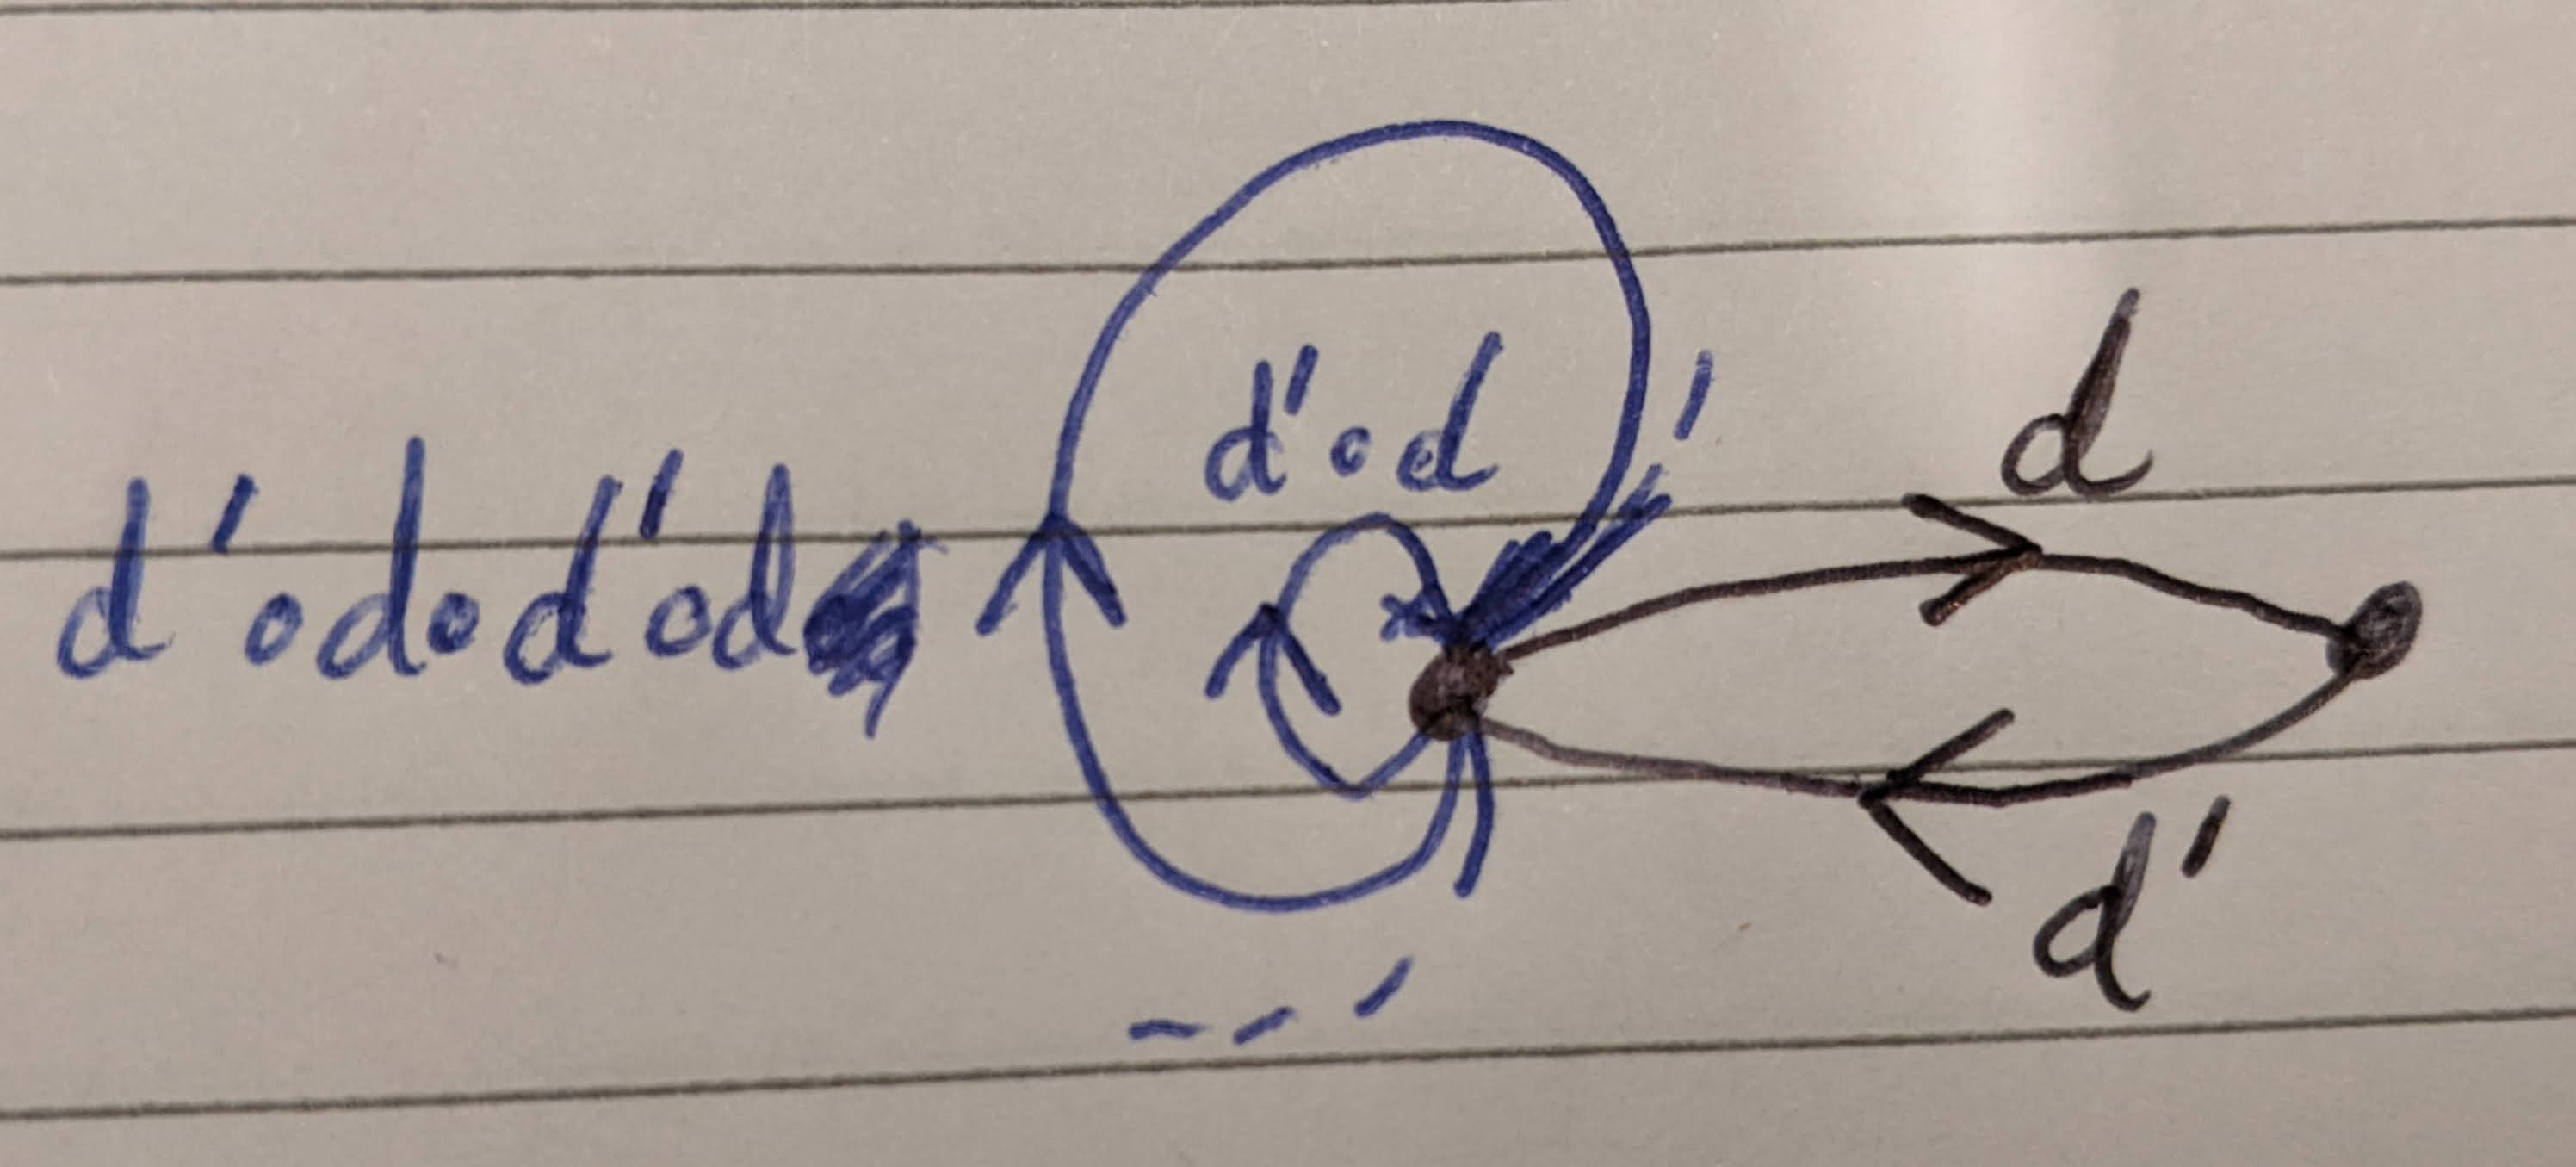
\includegraphics[width=1.0\linewidth]{2MathematicalFramework/InitialFramework/Images/D_commonly_large.jpg}
    % \captionof{figure}{Test caption.}
    \caption{A world diagram showing sequences of the transformations $d$ and $d'$ that are of the form $(d' \circ d)^{n}$.}
\end{center}
}, we do not show all the transformations in $D$ in our world diagrams unless explicitly stated.

Let's look at some world diagrams show casing some of the properties we've already seen.

\begin{figure}[H]
    \centering
    \begin{subfigure}[b]{0.45\linewidth}
        \centering
        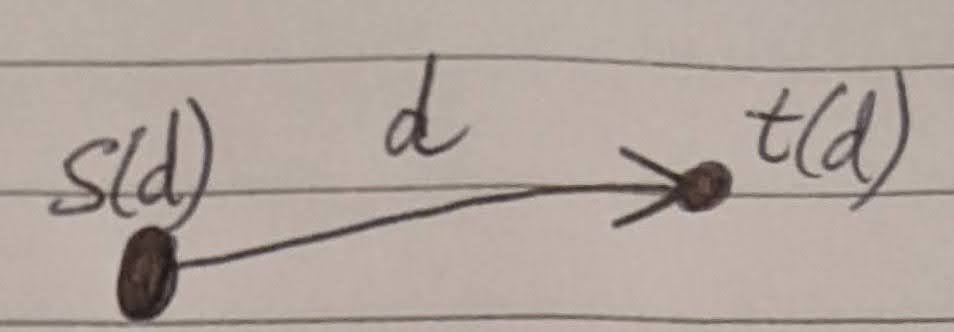
\includegraphics[width=\linewidth]{2MathematicalFramework/InitialFramework/Images/transformation.jpg}
        \caption{A wold diagram showing a transformation.}
        \label{fig:transformation}
    \end{subfigure}
    \hfill
    \begin{subfigure}[b]{0.45\linewidth}
        \centering
        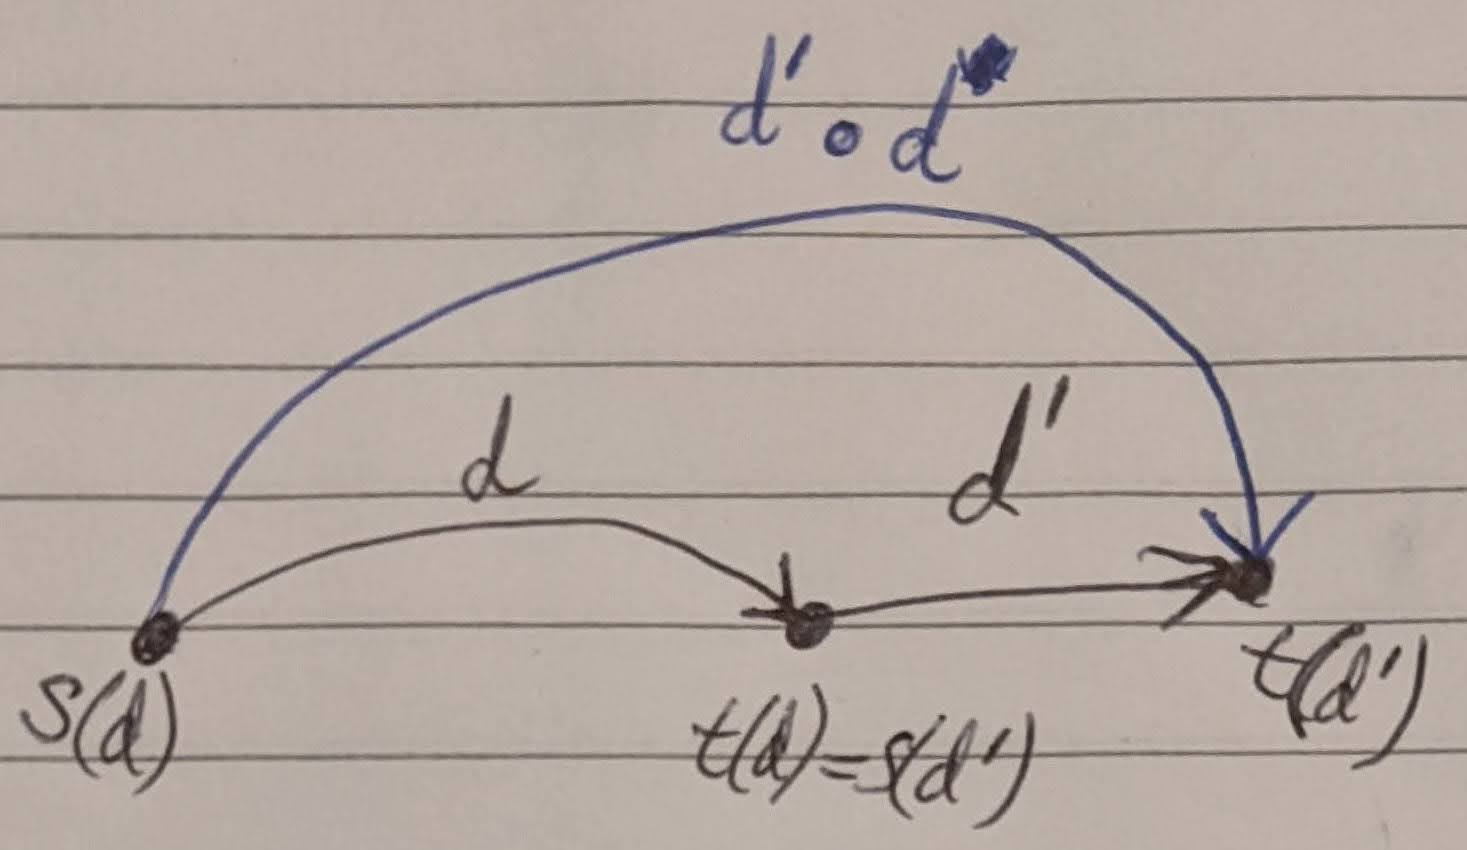
\includegraphics[width=\linewidth]{2MathematicalFramework/InitialFramework/Images/transformation_composition.jpg}
        \caption{A world diagram showing the composition of two transformations $d$ followed by $d'$ to give a transformation $d' \circ d$.}
        \label{fig:transformation_composition}
    \end{subfigure}
    \vskip\baselineskip
    \begin{subfigure}[b]{0.45\linewidth}
        \centering
        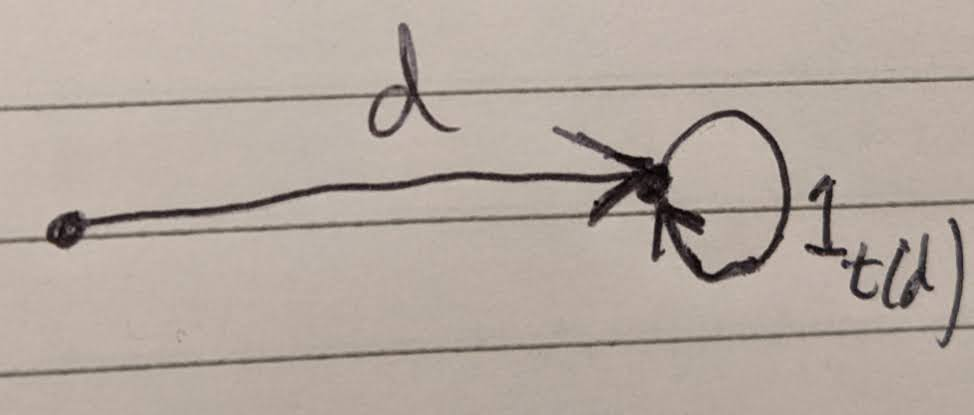
\includegraphics[width=\linewidth]{2MathematicalFramework/InitialFramework/Images/left_trivial_transformation.jpg}
        \caption{A world diagram showing a transformation $d: s(d) \to t(d)$ and its left identity element $1_{t(d)}$. Composing these two transformations gives the transformation $d$.}
        \label{fig:left_trivial_transformation}
    \end{subfigure}
    \hfill
    \begin{subfigure}[b]{0.45\linewidth}
        \centering
        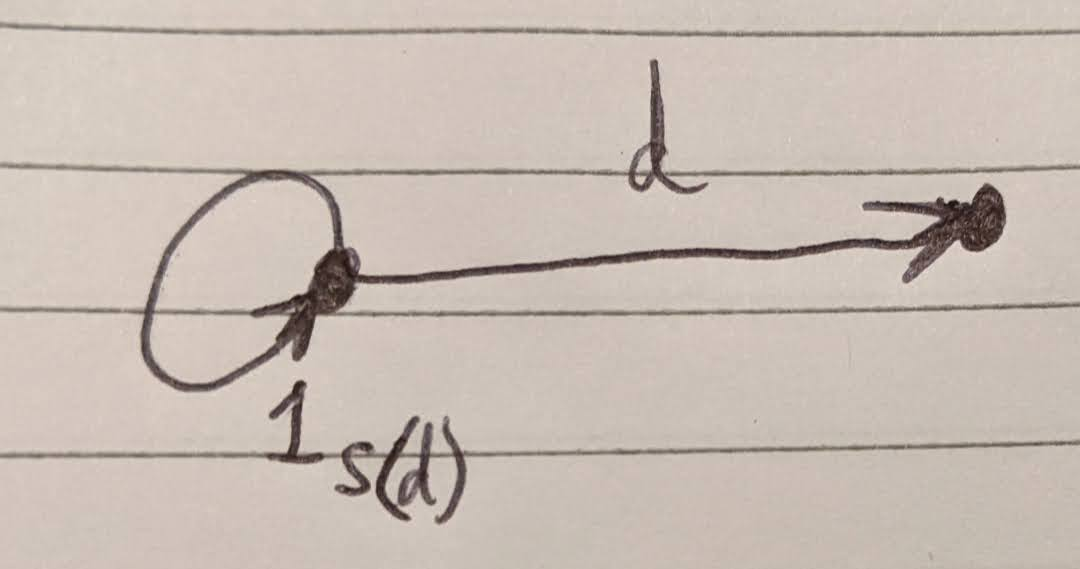
\includegraphics[width=\linewidth]{2MathematicalFramework/InitialFramework/Images/right_trivial_transformation.jpg}
        \caption{A world diagram showing a transformation $d: s(d) \to t(d)$ and its right identity $1_{s(d)}$. Composing these two transformations gives the transformation $d$.}
        \label{fig:right_trivial_transformation}
    \end{subfigure}
    \vskip\baselineskip
    \begin{subfigure}[b]{0.45\linewidth}
        \centering
        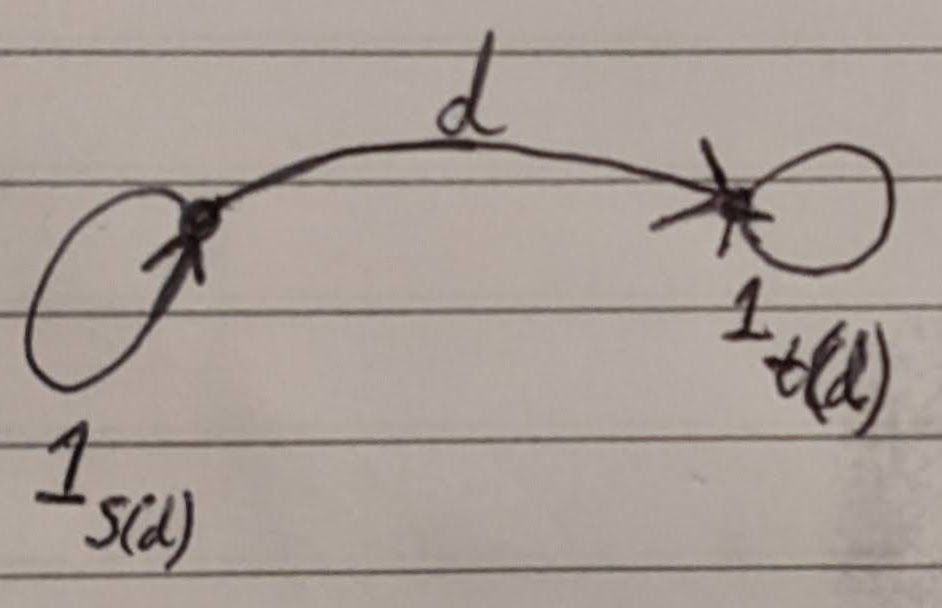
\includegraphics[width=\linewidth]{2MathematicalFramework/InitialFramework/Images/trivial_transformations_example_all_transformations.jpg}
        \caption{A world diagram showing a transformation $d: s(d) \to t(d)$, its left identity $1_{t(d)}$, and its right identity $1_{s(d)}$.}
        \label{fig:trivial_transformations_example_all_transformations}
    \end{subfigure}
    \caption{Examples of world diagrams displaying some of the concepts we have already come across.}
\end{figure}

It's important to note that, in a world diagram, the positioning (relative or absolute) of the world states and the shapes and lengths of the arrows do not matter\footnote{Formally, two world diagrams are isomorphic if...}:
\begin{figure}
    \centering
    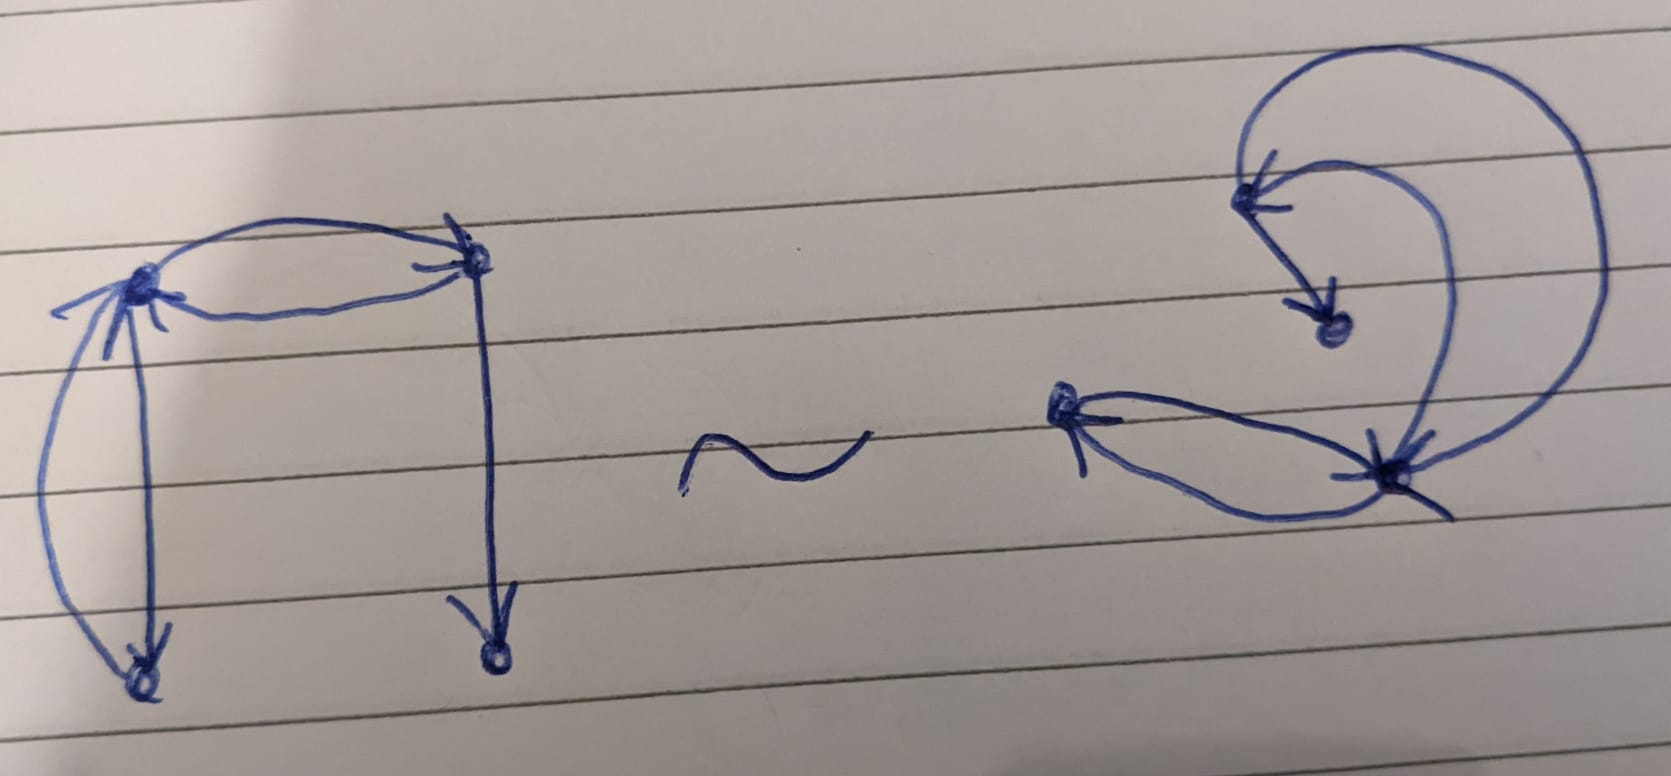
\includegraphics[width=0.5\linewidth]{2MathematicalFramework/InitialFramework/Images/isomorphic_world_diagrams.jpeg}
    \caption{The properties of these world diagrams are the same (the world diagrams are isomorphic).}
    \label{fig:isomorphic_world_diagrams}
\end{figure}

\paragraph{Subworlds.}
A world $\mathscr{W}' = (W', \hat{D}', \hat{s}', \hat{t}')$ is a \emph{subworld} of the world $\mathscr{W} = (W, \hat{D}, \hat{s}, \hat{t})$ if $W' \subseteq W$, $\hat{D}' \subseteq \hat{D}$, $\hat{s}' \subseteq \hat{s}$, and $\hat{t}' \subseteq \hat{t}$ \footnote{
This definition requires $\hat{D}' \subseteq \hat{D}$ and not $D' \subseteq D$ because removal of an element of $D$ which is not an element of $\hat{D}$ to create $D'$ would lead to sequences of minimum transformations not being transformations; to avoid problems like this we always consider the minimum transformations then use them to generate the set of transformations.
}.
We can denote that $\mathscr{W}'$ is a subworld of $\mathscr{W}$ using $\mathscr{W}' \subseteq \mathscr{W}$.
A subworld is a world.

\paragraph{Reachable and unreachable worlds.}
A world $\mathscr{W}'$ is \emph{reachable} from a world $\mathscr{W}$ if there exists a transition $d: w \to w'$ where $w \in W$ and $w' \in W'$ 
\footnote{
A sensible question is `what set of transformations contains $d$ ?'.
If $\mathscr{W}' \subseteq \mathscr{W}$ then $d \in \mathscr{W}$.
If $\mathscr{W}' \not\subseteq \mathscr{W}$ then we can consider a world $\mathscr{W}^{\aleph}$ containing all physically allowed world states and world state transformations; we then have that $\mathscr{W} \subseteq \mathscr{W}^{\aleph}$, $\mathscr{W}' \subseteq \mathscr{W}^{\aleph}$, and $d$ is an element of the set of transformations of $\mathscr{W}^{\aleph}$.
}.
If a world is not reachable, we say it is \emph{unreachable}.


We are building towards describing the structure of transformations in an agent's representation; late we will only be interested in the perspective of the agent and so will only care about the world states and transformations that the agent can come into contact with.
Unreachable and reachable worlds give us the language to describe and then disregard parts of worlds that agents will never explore and therefore are not relevant to the agent's representation.
For example, if an agent is in a maze and a section of the maze is inaccessible from the position that the agent is in, then that section of the maze would be disconnected from the section of the maze that the agent is in; if we want to study how the agent’s representation evolves as it learns, it makes sense to disregard world states where the agent is in the inaccessible part of the maze since those world states can never be reached and so those world states will not affect the agent's representation.
\footnote{
But what about worlds that are unreachable from the current world state, but the agent has already visited?
If we assume the representation evolution process is Markov, then all the necessary information will contained in the current representation space of the agent and so past world states which are now unreachable are irrelevant.
Therefore, for a Markov representation evolution process, we only need to consider the world states in subworlds that are reachable from the current world state.

If the representation evolution process is not Markov, we can transform the representation evolution process into a Markov process by augmenting the state space of the process to include any relevant historical information.
}
\begin{figure}
    \centering
    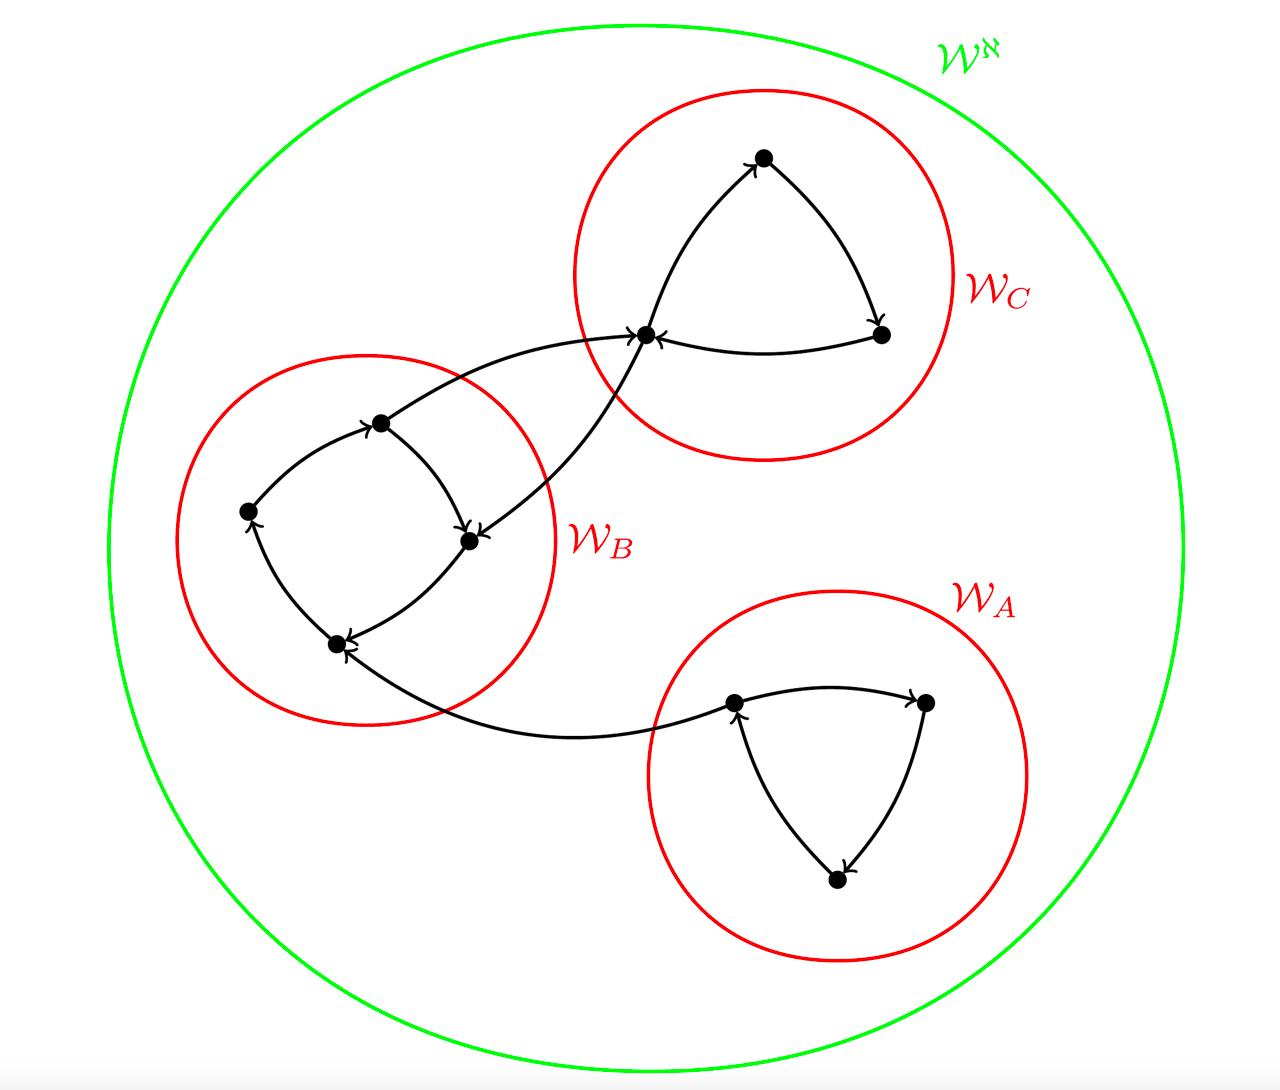
\includegraphics[width=0.5\linewidth]{2MathematicalFramework/InitialFramework/Images/reachable_worlds.jpg}
    \caption{
    $\mathscr{W}_{C}$ is reachable from $\mathscr{W}_{A}$ and $\mathscr{W}_{B}$, but $\mathscr{W}_{A}$ is not reachable from $\mathscr{W}_{B}$ or $\mathscr{W}_{C}$.
    }
    \label{fig:reachable_worlds}
\end{figure}

\whendraft{
\noindent\rule{\textwidth}{1mm}
\textbf{Small things:}
\begin{compactitem}
    \item \textbf{Mention:} we can have more than one minimum transformation between two states. Why we allow this becomes clear when we introduce the idea of agent actions.
    \item \textbf{Footnote:} Composition of transformations is read from left to right; the reason for this will be explained later.
    \item \textbf{Mention:} sometimes we don't include the trivial transformations for clarity.
    \item \textbf{Mention:} For the rest of this document, if we talk about a sets $D$, $\hat{D}$ of transformations or sets $W$ of worlds without explicitly defining an associated world $\mathscr{W}$, then the results are for a general world $\mathscr{W}$; we will explicitly define the world for specific examples.

    \item \textbf{Diagrams:}
        \begin{enumerate}
            \item (?) No unique element in $D$ for sequence with trivial transformations.
        \end{enumerate}
\end{compactitem}
\noindent\rule{\textwidth}{1mm}
}

%%%%%%%%%%%%%%%%%%%%%%%%%%%%%%%%%%%%%%%%%%%%%%%%%%%%%%%%%%
\section{Introducing an agent}
\newthought{We want to} study the structure of the representations of an agent that can interact with our worlds - we will now explain what an agent is in our framework.

\subsection{What is an agent ?}

\newthought{An \emph{agent} is} an autonomous entity\footnote{This could be a natural or artificial entity.} that can observe and interact with its environment\footnote{Our agent does not need to be embodied in the world - more on this later !}; the agents that we care about can also learn about their environments.

\subsection{Representations of an agent}

\newthought{An agent's \emph{representation states}} are the agent's internal representations of world states, through which the agent maintains its understanding of its world.
An agent's \emph{representation model} is the agent's internal model of the world, which includes how the agent encodes and organises information about its environment (e.g., as vectors, symbols, or other data structures) as representation states as well as the dynamics of how those representation states change due to actions that affect the world\footnote{The agent's representation model does not encode the dynamics of the world states, it encodes the dynamics of the representation states; a `good' representation will provide a good approximation to the dynamics of the world states. More on this later.}.

An agent's \emph{representation model} not only captures the current state of the world but also allows it to (attempt to) conceptualise future states by predicting the state of the world based on its observations and actions and plan actions accordingly, forming a comprehensive framework for decision-making and interaction.

\newthought{Agents use \emph{sensors}} to capture data from their world, enabling the agent to perceive the world; these sensors include real-world sensors (e.g., cameras on a robot, the human eye) and virtual inputs (e.g., data streams, user commands) in a software agent.
Sensors provide the agent with \emph{observation states}\footnote{Sometimes these are called sensory states such as in \cite{Ramstead2020}.}, which are the agent's internal representations of the information the sensors collect (e.g., data streams from the camera), and importantly are not the sensors themselves.
An \emph{agent's perceptual model} is how the agent encodes and organises information from its sensors (e.g., vectors, symbols, or other data structures) as well as how it conceptualises the structure of the landscape of possible observation states.

\newthought{Agents use \emph{effectors}} to interact with and alter their world, enabling the agent to carry out actions on the world; this can involve real-world effectors (e.g., motors and actuators on a robot) or virtual outputs (e.g., API calls or applying a transformation to a dataset the agent is manipulating) in a software agent.
These effectors receive \emph{effector signals}\footnote{Also known as \emph{control signals} in the field of robotics.}, which are the concrete instructions sent by the agent to execute actions (e.g., a voltage spike to a motor or a command to a software interface).
An agent also has an \emph{action model}, which is how the agent encodes and organises information about its actions (e.g., control signals, symbolic commands) as well as how it conceptualises how its actions will affect the world state.

An agent's action model is intrinsically linked to its representation model since the action model describes the movement between states of the representation model due to actions\footnote{These actions do not have to be only the actions of the agent itself, it can be a grouping of world state transformations that the agent understands to be from a particular cause - more on this later.}.

\whendraft{
\noindent\rule{\textwidth}{1mm}
\textbf{Additions:}
\begin{enumerate}
    \item \textbf{Figures:}
    \begin{itemize}
        \item Diagram showing what $W$, $Z$, $A$, $w$, $z$, $a$ are.
        \item Diagram showing mapping from $W$ to $O$ to $Z$.
    \end{itemize}
\end{enumerate}
\noindent\rule{\textwidth}{1mm}
}


\subsection{Agents as Markov blankets}

In our framework, we consider agents to be systems with internal states that interact with the world in ways that maintain a boundary between their internal states and the world.

Agent's in our framework have four types of state:
\begin{enumerate}
    \item \emph{Observation states} represent the agent's inputs from the environment (e.g., vision, sound, touch etc...).
    \item \emph{Effector states} represent how the agent influences the world state (i.e., the agent's external environment).
    \item \emph{(External) world states} consist of the states of the agent's external environment, which are the world states we introduced in section \ref{sec:A mathematical treatment of worlds and their transformations}.
    \item \emph{Agent's (internal) representation states} contain our agent's representations of the environment, memory model, knowledge models, goals, decision making processes etc...
    These internal states can only interact with the external world states via observation states and effector states.
\end{enumerate}

Using these four types of states we can view our agents as Markov blankets (see figure \ref{fig:markov_blanket}).

\begin{figure}
    \centering
    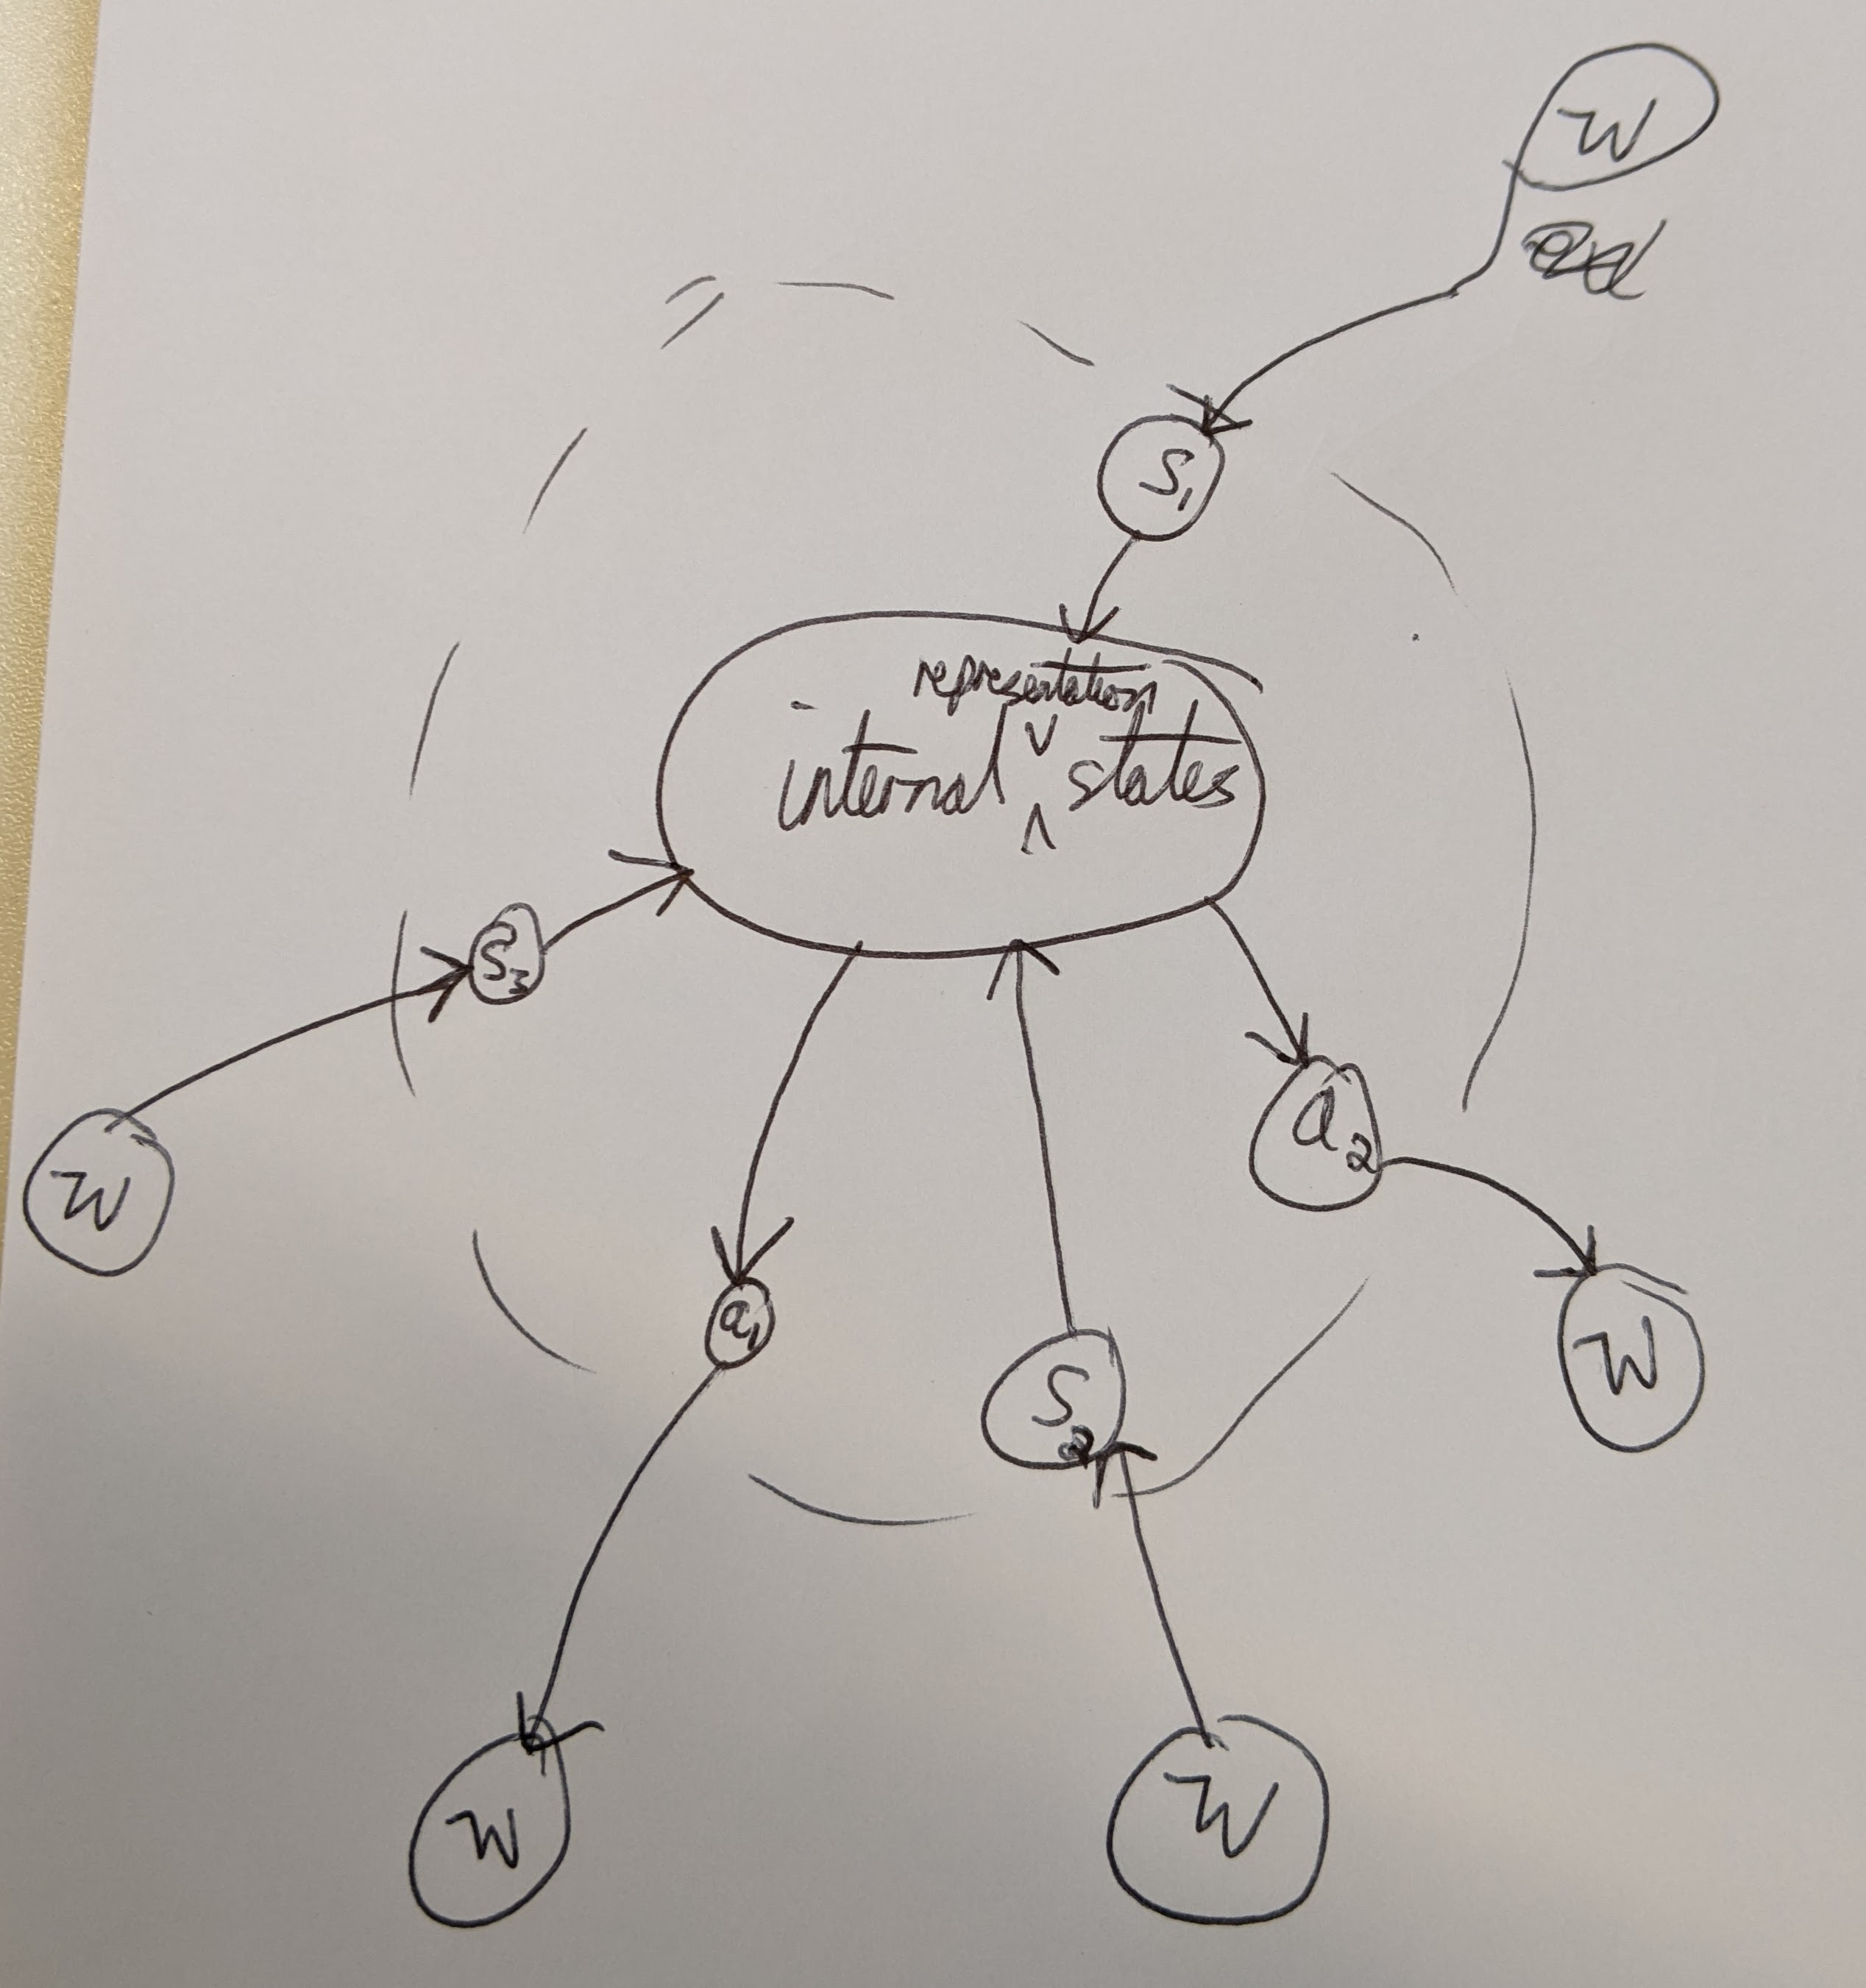
\includegraphics[width=0.5\linewidth]{2MathematicalFramework/InitialFramework/Images/markov_blanket.jpg}
    \caption{
    Complete caption.
    Arrows show the flow of information.
    }
    \label{fig:markov_blanket}
\end{figure}

The Markov blanket consists of the states that mediate interactions between our agent and its environment (the world) \cite{Ramstead2020}.

For our agent, the observation and effector states form the Markov blanket with the world states being outside the blanket and the the internal state being inside the blanket.
This Markov blanket acts as a boundary that separates the agent's internal representation states from the external world states.
The agent can not directly access the external world states, but can infer these world states by processing sensory inputs through its observation states and performing actions through its effector states; information about the world states crosses the Markov blanket through the agent's sensory states and the agent's affect on the world crosses the Markov blanket through the agent's effector states.

Technically, given the observation and effector states (i.e., the blanket), the internal representation states of the agent are \emph{conditionally independent} of the external world states; conditionally independent of the external world states means that the behaviour of the agent's internal representation depends only on the states of the agent's Markov blanket (i.e., the agent's observation and effector states) and not (directly) on the world states external to the agent because all the relevant information about the external world states are filtered through the observation states and the agent only affects the world through its effector states.

By framing an agent as a Markov blanket, we clearly show that the agent learns about its world only through its observation states and its actions.
One major implication of this approach for our framework is we consider the internal representation states of the agent to be separate from the world states introduced in section \ref{sec:A mathematical treatment of worlds and their transformations}; this means that if we swap an agent embodied in a world with another agent that is identical except for having a different internal representation state (or a different representation model), then the world state would remain unchanged.

Another implication is that, since an agent's only gains knowledge about the strucutre of the world through its sensors and its actions, world states with differences that are not detectable by the agent are identical from the agent's perspective and so can be treated as such when we are constructing a mathematical description of the agent's interaction with the world (i.e, those world states do not exist from the perspective of the agent)\footnote{More on this later !}.

\subsection{Sensory perception}

Our agents have an unspecified number of sensors that allows it to make observations of the world.
Information about the agent's current world state is delivered to the internal state of the agent as an observation state; this is called the \emph{observation process}\footnote{If the world state is modelled as a distribution then is process is also referred to as the agent \emph{sampling} the world state.}.
For example, the human eye (the sensor) converts information about the light entering the eye into
electrical and chemical energy in the optic nerve (the observation process).

Mathematically, we treat the observation process as a mapping $b: W \to O$ which produces an observation $o_{i}$.
The structure of $o_{i}$ depends on the agent's perceptual model; commonly, each observation $o_{i}$ is a vector of length $N$, where $N$ is the number of sensors the agent has.

\begin{figure}
    \centering
    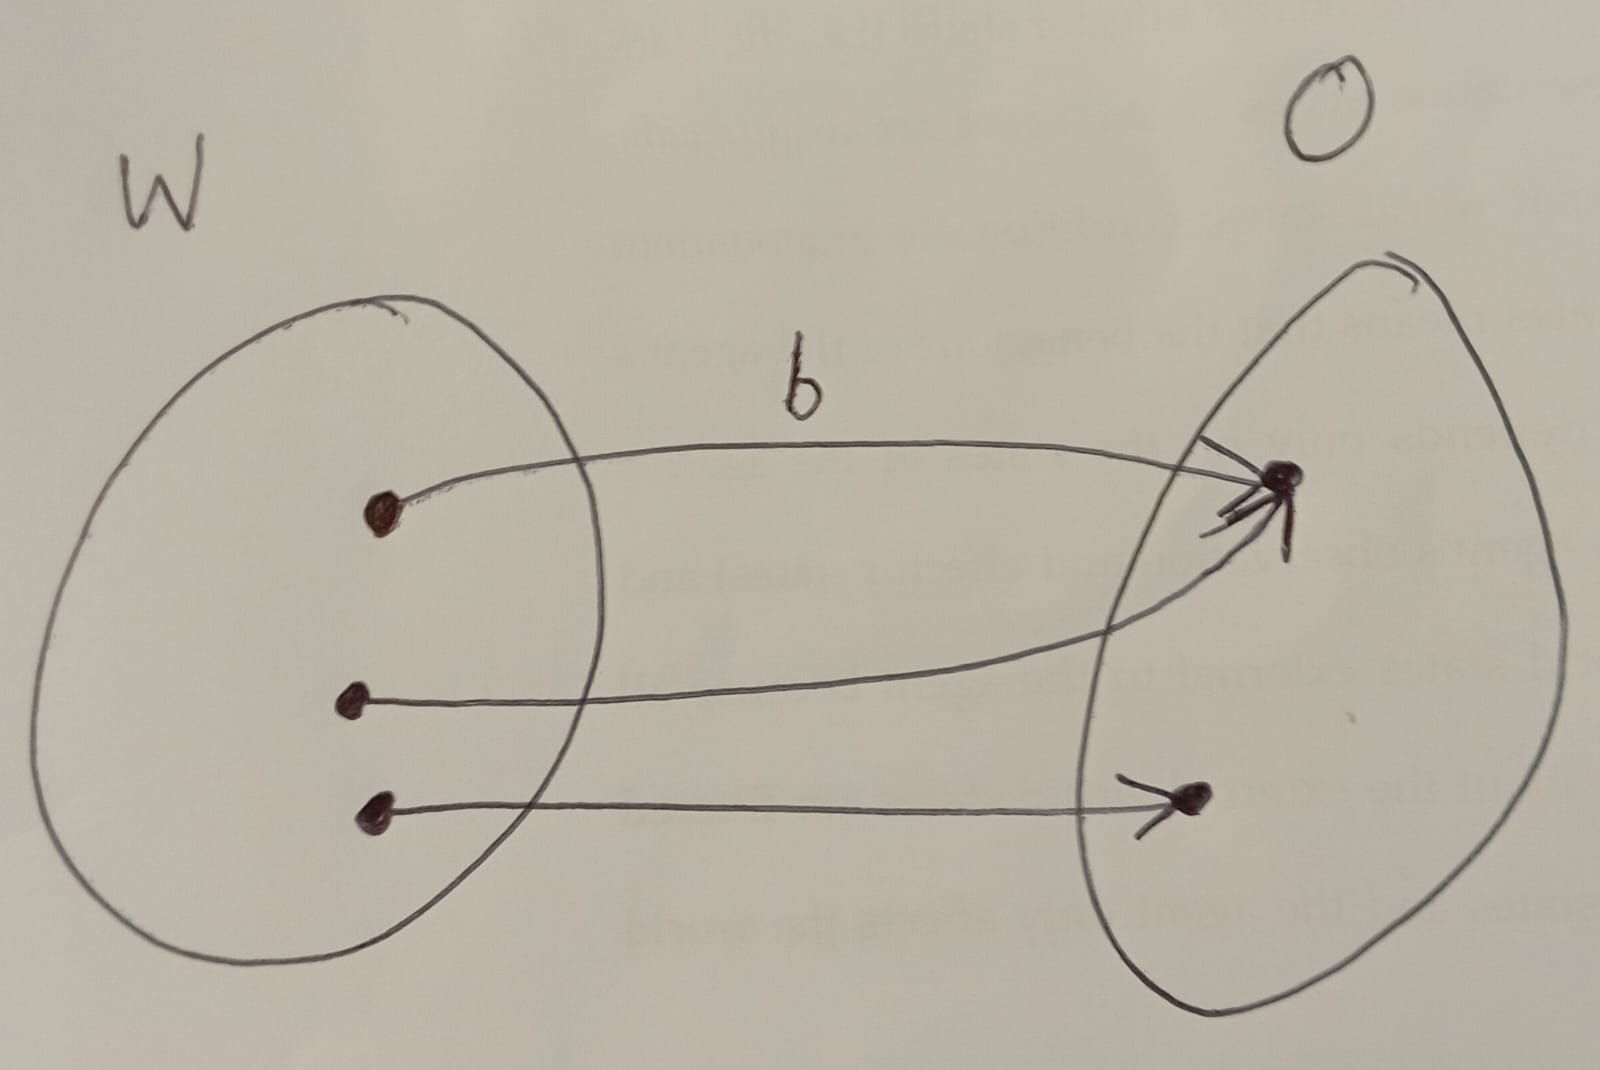
\includegraphics[width=0.5\linewidth]{2MathematicalFramework/InitialFramework/Images/observation_process_W_to_O.jpeg}
    \caption{Caption}
    \label{fig:observation_process_W_to_O}
\end{figure}

Initially, we will consider our agents to have \emph{perfect sensors}; for an agent with perfect sensors:
\begin{enumerate}
    \item information is not lost or modified during the observation process,
    \item there is no noise in the sensors, 
    \item a change in the world state causes a change in the observation state\whendraft{\footnote{This might be too strict? We want to allow cases where $b(w_{1})=b(w_{2})$ due to things such as occlusion? Should we discuss this separately later or should we introduce something like a world with bijective f ?}}.
\end{enumerate}

In real world situations, it is common for information about the world state to be lost, modified or not picked up during the observation process; for example, the human eye only picks up certain wavelengths of light or a camera could take in a colour spectrum then output greyscale.
We will discuss agents with non-perfect sensors in section ???.

Something else to note is that world states with differences that are not detectable by the agent's sensors or actions are effectively identical from the agent's perspective and so can be treated as such when we are constructing a mathematical description of the agent's interaction with the world.

\subsection{Learning and inference}

We consider agents that learn about their world.
The end goal of the agent’s learning process is to map the useful aspects of the structure of the world to the structure of its representation; the useful aspects are those that enable the agent to complete whatever task the agent has.
The observation states from our agents' sensors are used by an \emph{inference process} to produce a representation of the current state of the world; the agent
then uses some internal mechanism to select an action to perform.
For example, the electrical signals from the optic nerve are given to the brain for inference; mechanisms in the brain then select an action to be performed. 
Mathematically, we consider this inference process to be a mapping $h: O \to Z$.
\begin{figure}
    \centering
    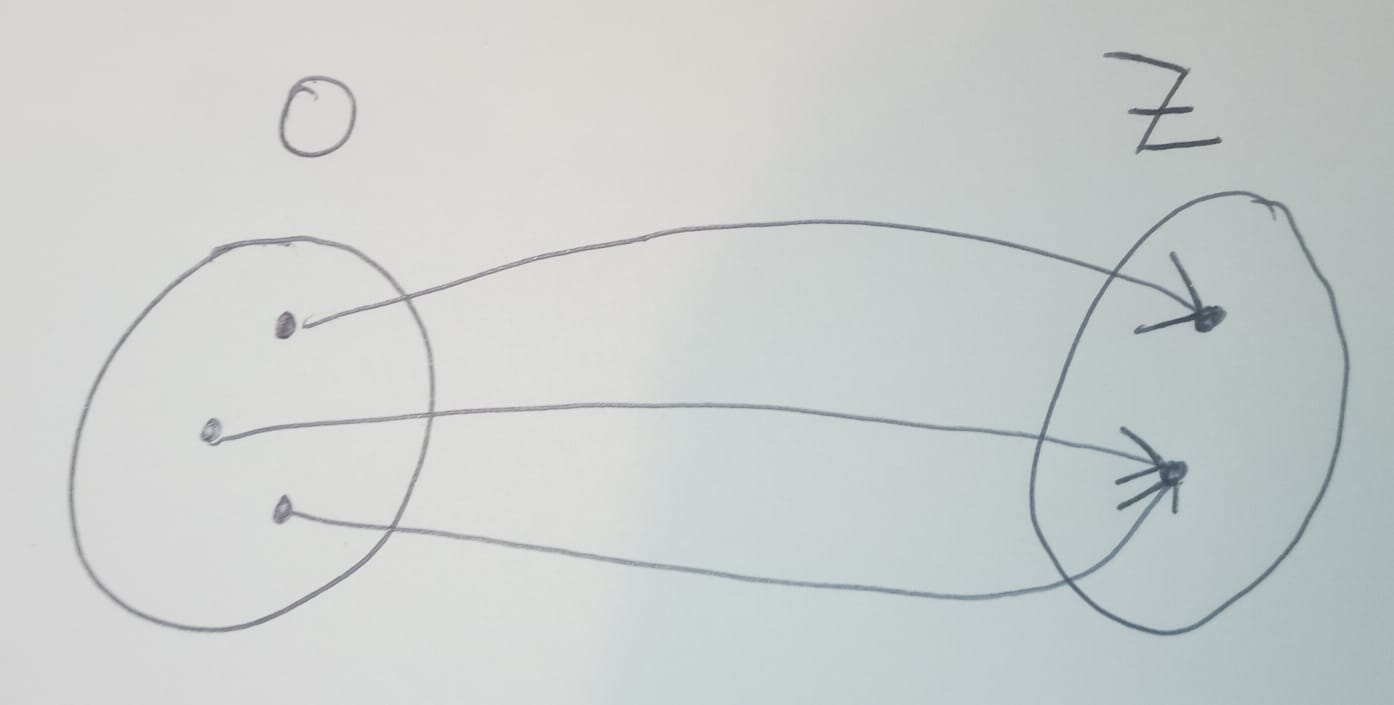
\includegraphics[width=0.5\linewidth]{2MathematicalFramework/InitialFramework/Images/inference_process_O_to_Z.jpeg}
    \caption{Caption}
    \label{fig:inference_process_O_to_Z}
\end{figure}

For agents without perfect sensors, there are scenarios (e.g., in partially observable environments) where two world states that are distinct for the agent produce the same observation state (i.e., $h(o_{\alpha}) = w_{1}$ and $h(o_{\alpha}) = w_{2}$).
We will discuss these types of scenarios in section ???.

For agents with perfect sensors, we can combine $b$ and $h$ to form a mapping $f = h \circ g$ from $W$ to $Z$\whendraft{\footnote{\textbf{Proof that this map always exists if agent perfect sensors ?}}}.
We will initially focus on the structure of an agent's representation due to these types of maps $f$.
\begin{figure}
    \centering
    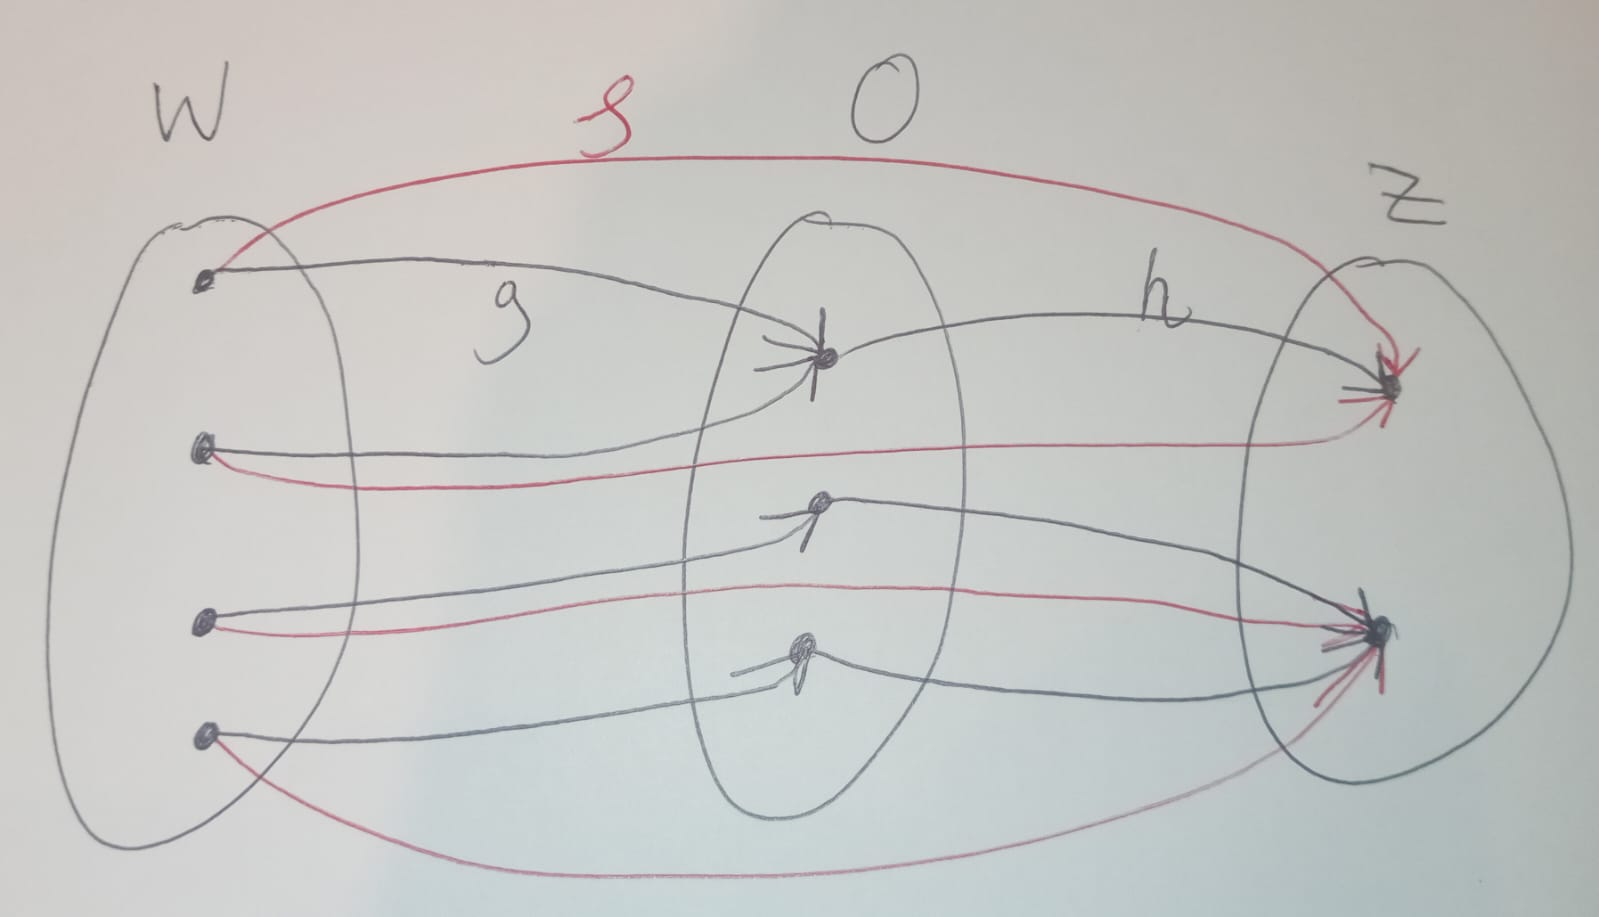
\includegraphics[width=0.5\linewidth]{2MathematicalFramework/InitialFramework/Images/W_to_Z.jpeg}
    \caption{Caption}
    \label{fig:W_to_Z}
\end{figure}


\subsection{Our approach}

We propose there are two approaches for understanding the learning of an agent: (1) we can study the learning process of the agent itself (i.e., how does the agent learn at each step of the learning process) or (2) we can study what we believe the end result of the agent's learning process should be.
We will initially focus on approach (2).

We assume that the best representation of the worlds we study should exactly mirror the structure of the worlds themselves in the structure of the agent's representation, and so the end result of the agent's learning process should be
By initially studying the structure of worlds themselves, rather than structure of an agent's representation, we simplify the problem we are tackling since we no longer have to consider each step of the learning process; this provides the opportunity to generalises our results somewhat - for example, if we prove that the structure of the world does not obey certain conditions then we might be able to show that this is true no matter the process used for learning\whendraft{\footnote{\textbf{Flesh this out a bit more - talk about learning equilibria ?}}}.

Once we have this foundation, we can introduce aspects of non ideal sensors to see how they affect the agent's representation when learning the structure of the same worlds we've already studied.

\whendraft{
\noindent\rule{\textwidth}{1mm}

\textbf{Up next:}
\begin{enumerate}
    \item Sensory perception in an agent.
    \begin{compactitem}
        \item Look at Higgins distribution set up.
        \item Cones figure - cone in $W$ leading to a single observation in $O$ - put in later discussion.
        \item If the agent's sensors are perfect (i.e., there is no noise from the sensors) the number of possible observation states is less than or equal to the number of world states (i.e., $|O| \leq |W|$) - put this should later with a proof.
    \end{compactitem}

    \item Learning.
    \begin{compactitem}
        \item Brief discussion about scenarios where you can have $b(w_{1}) = b(w_{2})$ but $h(b(w_{1})) \neq h(b(w_{2}))$ - say we'll discuss this in more detail later.
        \item Proof that the structure of an agent's representation should mirror the structure of the agent's representation for an agent with ideal sensors.
    \end{compactitem}
\end{enumerate}

\textbf{Small things:}
\begin{compactitem}
    \item Environment vs world.
    \item Mention at start of Agents section that we use a mix of papers for inspiration for our agent: Agent as a Markov blanker paper, Higgins, Caselles-Dupre.
    \item World states as a distribution - see Higgins.

    \item \textbf{Diagrams:}
        \begin{enumerate}
            \item 
        \end{enumerate}

    \item \textbf{References:}
    \begin{enumerate}
        \item Agent as a Markov blanket: \url{https://www.researchgate.net/figure/The-structure-of-a-Markov-blanket-A-Markov-blanket-highlights-open-systems-exchanging_fig1_343643283}
    \end{enumerate}
\end{compactitem}


\textbf{Implemented notes:}
\begin{compactitem}
    \item Do the 'sensory states' in the Markov Blanket represent different observation states in $O$ or different sensors ? They represent different observation states - need to make my formalism consistent. \textbf{Use $o$ for observation states.}
    \item Sensors can mean real-world sensors or virtual inputs (e.g., in a software agent).
\end{compactitem}
\noindent\rule{\textwidth}{1mm}
}

%%%%%%%%%%%%%%%%%%%%%%%%%%%%%%%%%%%%%%%%%%%%%%%%%%%%%%%%%%%%%%%%%%%
\section{Actions of agents}

In this section, we define the actions of agents as collections of transformations that are labelled by their associated action, and then we define some relevant properties of these actions.

%%%%%%%%%%%%%%%%%%%%%%%%%%%%%%%%%%%%%%%%%%%%%%%%%%%%%%%%%%%%%%%%%%%
\subsection{Actions as collections of labelled transformations}

Consider a set $\hat{A}$ called the set of \emph{minimum actions} of an agent, where $\hat{A} = \{1, a_{1}, a_{2}, \dots, a_{n}\}$.

We now take the Kleene star operator of $\hat{A}$ \footnote{
$\hat{A}^{*} = \{ \epsilon \} \cup \{ (a_1, a_2, \dots, a_n) \mid a_i \in \hat{A}, \, n \in \mathbb{N} \}$.
} to get the set of all possible finite sequences formed from elements of $\hat{A}$, including the empty sequence $\epsilon$.
We call $\hat{A}^{*}$ the set of \emph{actions} of an agent.

We define a composition operator $\circ: \hat{A}^{*} \times \hat{A}^{*} \to \hat{A}^{*}$ such that $(a_1, a_2, \dots, a_n) \in \hat{A}^{*}$ can be written as $a_1 \circ a_2 \circ \dots \circ a_n$.
Sometimes we write compositions like $a_1 \circ a_2 \circ \dots \circ a_n$ as $a_1 a_2 \dots a_n$.
The operator $\circ$ is closed under the definition of the Kleene star operator.

\paragraph{Properties of the empty sequence $\epsilon$.}
\begin{enumerate}
    \item \textbf{Uniqueness:} There is only one empty sequence $\epsilon$.
    \item \textbf{Identity element for concatenation:} the empty sequence $\epsilon$ serves as an identity element for concatenation of sequences:
    $\epsilon \circ a = a \circ \epsilon = a$ for all $a \in \hat{A}^{*}$.
    \item \textbf{Length:} The empty sequence $\epsilon$ has a length of zero (i.e., $|\epsilon| = 0$).
\end{enumerate}

\paragraph{Linking actions with transformations.}
We now want to link our set of actions to the transformations of the world that would occur if an agent performed each action while in a current world state.
We do this by first labelling transformations in the set $D$ of transformations that are caused by minimum actions with the elements of $\hat{A}$, and then using those labellings to label other transformations in $D$ with the elements of $\hat{A}^{*}$ by considering how the elements of $\hat{A}$ combine to form the elements of $\hat{A}^{*}$.

Consider a set $\hat{D}_{A} \subset D$, where $1_{w} \in \hat{D}_{A}$ for all $w \in W$; we call $\hat{D}_{A}$ the set of \textit{minimum action transformations}.
We define a labelling map $\hat{l}: \hat{D}_{A} \to \hat{A}$ such that:
\begin{enumerate}
    \item Any two distinct transformations leaving the same world state are labelled with different actions.
    \begin{action_condition}\label{actcon:action_gives_single_outcome}
        For any $d,d' \in \hat{D}_{A}$ with $s(d)=s(d')$, $\hat{l}(d) \neq \hat{l}(d')$.
    \end{action_condition}

    \item Trivial transformations, $1_{w}$ for all $w \in W$, are mapped by $\hat{l}$ to the empty sequence $\epsilon$:
    \begin{action_condition}\label{actcon:trivial_transformations_mapped_to_empty_sequence}
        $\hat{l}(1_{w}) = \epsilon$ for all $w \in W$.
    \end{action_condition}
\end{enumerate}

So, for any world $\mathscr{W} = (W, \hat{D}, \hat{s}, \hat{t})$, there is a subworld $\mathscr{W}_{A} = (W, \hat{D}_{A}, \hat{s}, \hat{t})$.
In the same way as we did in section \ref{sec:A mathematical treatment of worlds and their transformations} to get $D$ from $\mathscr{W}$, we take the set of all paths in $\mathscr{W}_{A}$ and denote it by $D_{A}$; the elements of $D_{A}$ are called \emph{transformations due to the actions of the agent}.
As before, we extend $\hat{s}$ and $\hat{t}$ to $s$ and $t$ respectively\footnote{
We can use $s$, $t$ instead of having to define sub maps $s_{A}$ and $t_{A}$ because $s$ and $t$ act on the elements of $D$ and $D_{A}$ is just $D$ with some elements removed.
If we wanted to define such maps $s_{A}$ and $t_{A}$ they would be restrictions of the maps $s$ and $t$ to the set $D_{A}$.
\whendraft{
- Put this as a footnote for the definition of subworlds?
does this slightly alter the definition of subworld ?
}
}.

We extend the map $\hat{l}$ to the map $l: D_{A} \to \hat{A}^{*}$ such that:
if $d = \hat{d}_{n} \circ ... \circ \hat{d}_{1}$ then $l(d) = \hat{l}(\hat{d}_{n}) ... \hat{l}(\hat{d}_{1})$.

For $d \in D_{A}$ with $s(d) = w$, $t(d) = w'$ and $l(d) = a$, we will often denote $d$ by $d: w \xrightarrow{a} w'$.

\paragraph{Effect of actions on world states.}
Unlike transformations, which are tied to individual world states, actions can have different outcomes when applied to different world states.
For example, it could be the case that applying the action $a$ followed by the action $b$ on a world state $w_{1}$ gives back the original world state, while applying $a$ followed by $b$ on world state $w_{2}$ could give a different world state $w_{3}$ - the action sequence $ba$ produces the original world state when applied to certain world states (e.g., $w_{1}$), but produces a world state that is not the original world state when applied to other world states (e.g., $w_{2}$).
Due to this behaviour, we need a way to describe how actions change world states.
We define the \emph{effect of an action $a \in A$ on world state $w \in W$} as

\begin{itemize}
    \item[] $*: \hat{A}^{*} \times W \to W$ such that
    \begin{enumerate}[(1)]
        \item if there exists $d \in D_{A}$ such that $s(d) = w$ and $l(d) = a$, then $a * w = t(d)$, and
        \item if there does not exist $d \in D_{A}$ such that $s(d) = w$ and $l(d) = a$, then we say that $a * w$ is \emph{undefined}.
    \end{enumerate}
\end{itemize}
From now on, unless stated otherwise, when we give something like $a * w$ we will assume that $a * w$ is defined.

The effect of actions on world states is well-defined due to action condition \ref{actcon:action_gives_single_outcome}.

We can apply the minimum actions that make up an action to world states individually:
if $a = \hat{a}_{k}...\hat{a}_{1}$, then
\begin{align*}
    a * w &= (\hat{a}_{k} \dots \hat{a}_{1}) * w \\
          &= (\hat{a}_{k} \dots \hat{a}_{2}) * (\hat{a}_{1} * w) \\
          &= (\hat{a}_{k} \dots \hat{a}_{3}) * (\hat{a}_{2} * (\hat{a}_{1} * w)) \\
          &= \dots
\end{align*}

We can also apply split actions into short sequences of actions and apply those:
if $a = \hat{a}_{k}...\hat{a}_{1}$, then
\begin{align*}
    a * w &= (\hat{a}_{k} \dots \hat{a}_{3}) * (\hat{a}_{2} * (\hat{a}_{1} * w)) \\
          &= (\hat{a}_{k} \dots \hat{a}_{3}) * ((\hat{a}_{2} \hat{a}_{1}) * w) \\
          &= \dots
\end{align*}

\paragraph{Actions as (partial) functions.}

Consider all the transformations that are labelled by a particular action $a \in \hat{A}^{*}$.
Together these transformations form a partial function $f_{a}: W \to W$ because for any $w \in W$ either $a * w$ is undefined or $a * w$ is defined and there is a unique world state $w' \in W$ for which $a * w = w'$ (from action condition \ref{actcon:action_gives_single_outcome}).
Each of the transformations labelled by the action $a$ is an assignment of $f_{a}$ to one of the world states in $W$.
This function $f_{a}$:
\begin{itemize}[-]
    \item is not generally surjective because for a given $w \in W$ there is not necessarily a transition $d \in D$ with $l(d) = a$ and $t(d) = w$ \draftnote{blue}{awjdean}{Illustrative diagram},

    \item is not generally injective because it is possible to have an environment where $f_{a}(w)=f_{a}(w')$ for some $w \in W$ different from $w' \in W$ \draftnote{blue}{awjdean}{Illustrative diagram}.
\end{itemize}

Another way of thinking about this is we can take the action effect operator $* : \hat{A}^{*} \times W \to W$ and curry it\draftnote{blue}{awjdean}{reference} to give a collection $\{*_{a}\}$ of partial functions, where there is a partial function $\hat{*}(a)=*_{a}: W \to W$ for each action $a \in \hat{A}^{*}$:
\begin{equation*}
    \textit{Curry}: (*: \hat{A}^{*} \times W \to W) \to (*_{a}: W \to W)
\end{equation*}
\footnote{
We can also reproduce these functions using the formalism given by \autocite{caselles2019symmetry}, which describes the dynamics of the world in terms of a multivariate function $f: A \times W \to W$.
If we let $f: A \times W \to W$ be the dynamics of the environment then the transition caused by an action $a \in A$ on a world state $w \in W$ (where $a * w$ is defined) is given by $(a,w) \mapsto f(a,w) = a * w$. \draftnote{blue}{awjdean}{Put stuff like this in a separate "Other formalisms described using our formalism" section after Reproducing SBDRL ?}
}

\whendraft{
\noindent\rule{\textwidth}{1mm}
\textbf{Up next:}
\begin{enumerate}
    \item Example.
    \begin{compactitem}
        \item Diagram (l-map-for-transitions-from-and-to-w0).
        \begin{compactitem}
            \item This diagram shows how the minimum transitions $d$ with $d(s) = w_{0}$ or $d(t)= w_{0}$ are mapped to actions using the map $l$.
            \item Figure ref[fig:l-map-for-transitions-from-and-to-w0] demonstrates how the map $l$ maps transitions in $D$ to the elements in $A$ for the transitions shown in Figure \ref{fig:2x2-cyclical-min-actions-standard}.
        \end{compactitem}
    \end{compactitem}
\end{enumerate}

\textbf{To do:}
\begin{enumerate}
    \item Appendix: Why $\hat{A}$ is not necessarily labelling elements of $\hat{D}$ only.
    
    \item Is $l$ actually a collection of maps $l_{w}$ for each $w \in W$ ? --> endomorphism viewpoint ?

    \item Talk about why we've created action condition 1.
    \item \textbf{Footnote:} difference between the empty action and the no op action. 
    \item Say we refer to the empty sequence as the empty action.

    \item \textbf{Mention:} We can use $s$, $t$ instead of having to define sub maps $s_{A}$ and $t_{A}$ because $s$ and $t$ act on the elements of $D$ and $D_{A}$ is just $D$ with some elements removed. - Put this as a footnote for the definition of subworlds; does this slightly alter the definition of subworld ?

    \item \textbf{Mention:} Minimum actions denoted by $\hat{hat}$.

    \item No-op action doesn't always exist.
    \begin{compactitem}
        \item Physically, the identity action $1 \in A$ corresponds to the no-op action (\textit{i.e.}, the world state does not change due to this action).
    \end{compactitem}
\end{enumerate}

\textbf{Questions/thoughts that have been answered:}
\begin{compactitem}
    \item $A$ is the set of words made from $\hat{A}$ - i.e., the set of finite sequences of elements of $A$, not infinite sequences - infinite sequences make things tricky (apparently).

    \item We want the set $A$ of actions to be the Kleene star operation of $\hat{A}$ ($A = \hat{A}^{*}$). $\hat{A}^{*}$ includes an empty sequence $\epsilon$ and our no-op action $1$ as separate sequences; if the no op action is an identity action, then $1 \sim \epsilon$.
\end{compactitem}
}


\noindent\rule{\textwidth}{1mm}
%%%%%%%%%%%%%%%%%%%%%%%%%%%%%%%%%%%%%%%%%%%%%%%
\textbf{Example - agent in cyclical world}

We consider a cyclical $2\times 2$ grid world, denoted by $\mathscr{W}_{c}$, containing an agent as shown in Figure \ref{fig:2x2-cyclical-grid-world-states}.
The transformations of $\mathscr{W}_{c}$ are due to an agent moving either up ($U$), down ($D$), left ($L$), right ($R$), or doing nothing ($1$).
The possible world states of $\mathscr{W}_{c}$ are shown in Figure \ref{fig:2x2-cyclical-grid-world-states}.
$\mathscr{W}_{c}$, and variations of it, is used as a running example to illustrate the concepts presented in this paper.

\begin{figure}
    \centering
    \begin{subfigure}[b]{0.45\linewidth}
        \centering
        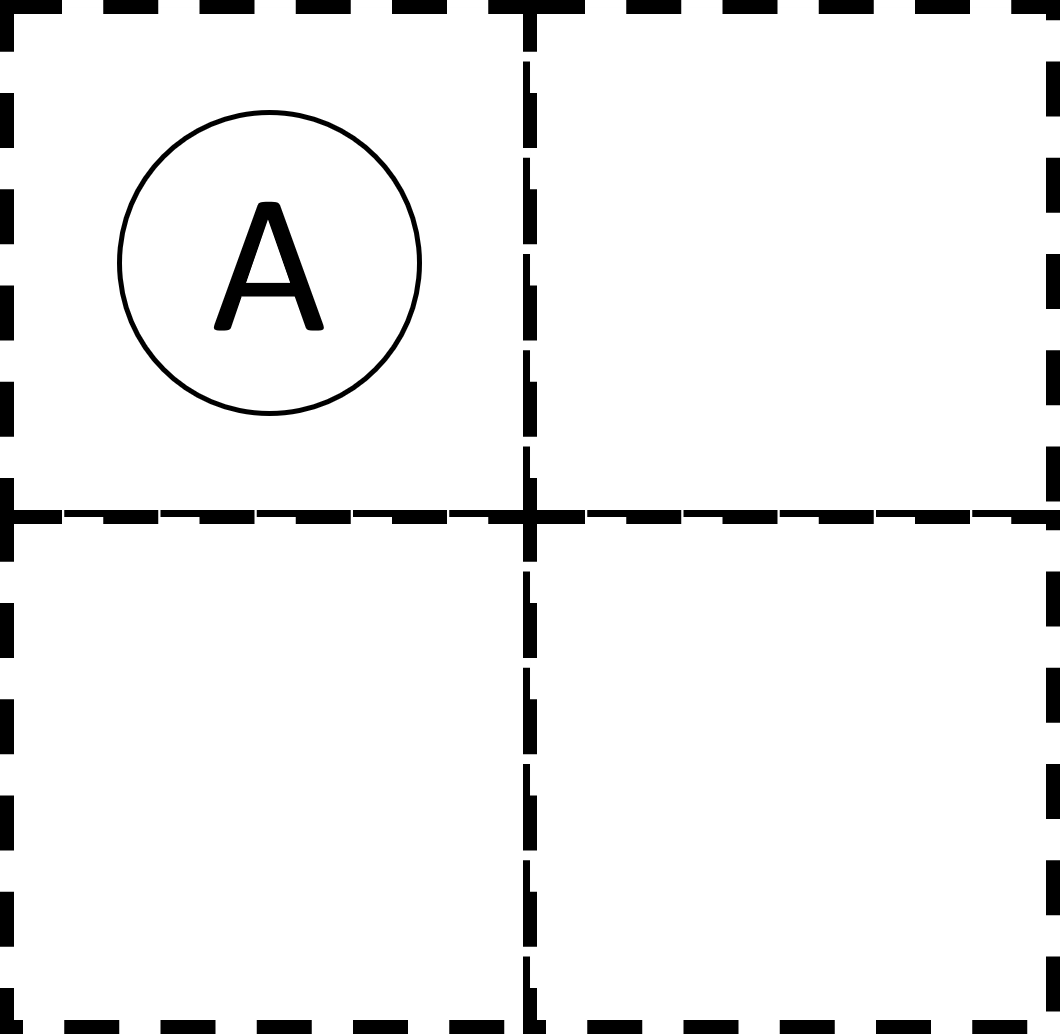
\includegraphics[width=0.5\linewidth]{2MathematicalFramework/InitialFramework/Images/2x2_no_walls_world_states/w0.png}
        \caption{$w_{0}$}
        \vspace{0.25cm}
    \end{subfigure}
    \begin{subfigure}[b]{0.45\linewidth}
        \centering
        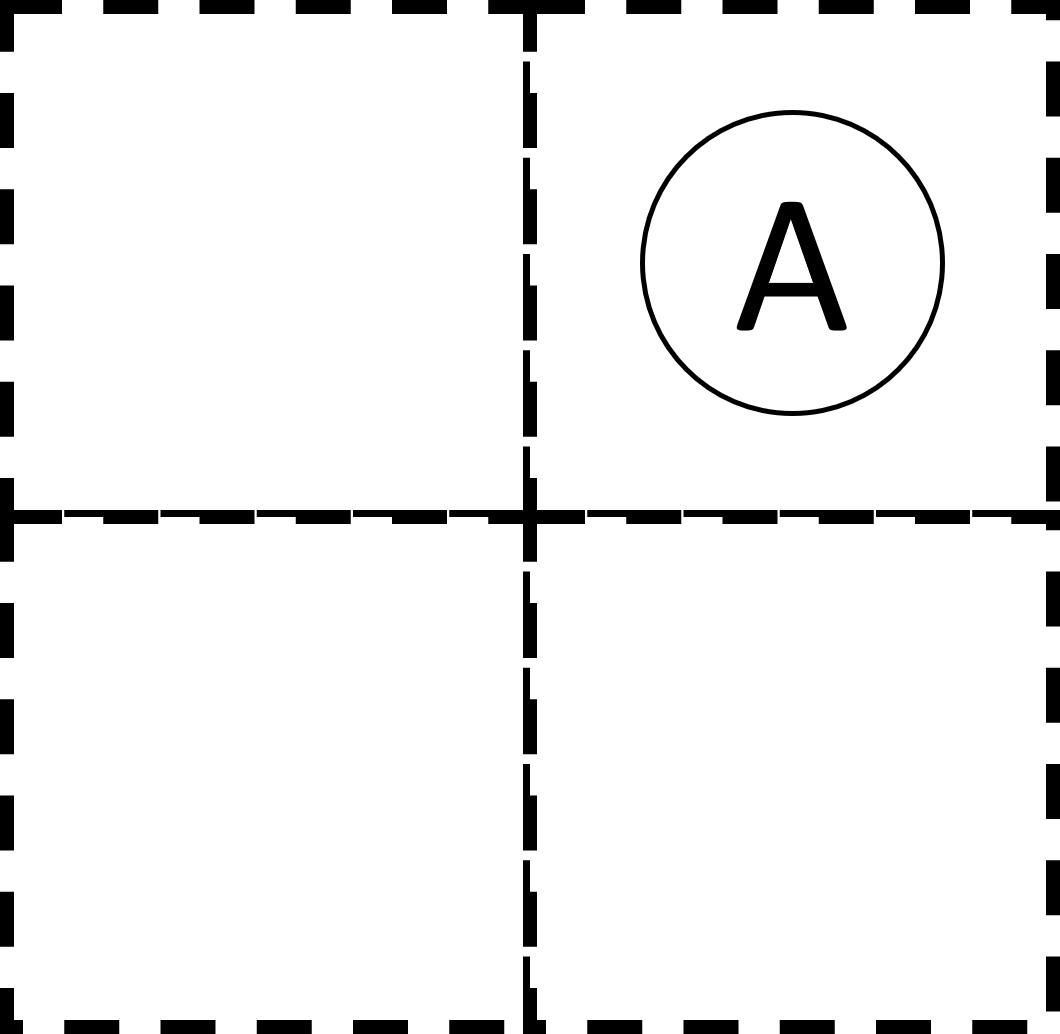
\includegraphics[width=0.5\linewidth]{2MathematicalFramework/InitialFramework/Images/2x2_no_walls_world_states/w1.png}
        \caption{$w_{1}$}
        \vspace{0.25cm}
    \end{subfigure}
    \begin{subfigure}[b]{0.45\linewidth}
        \centering
        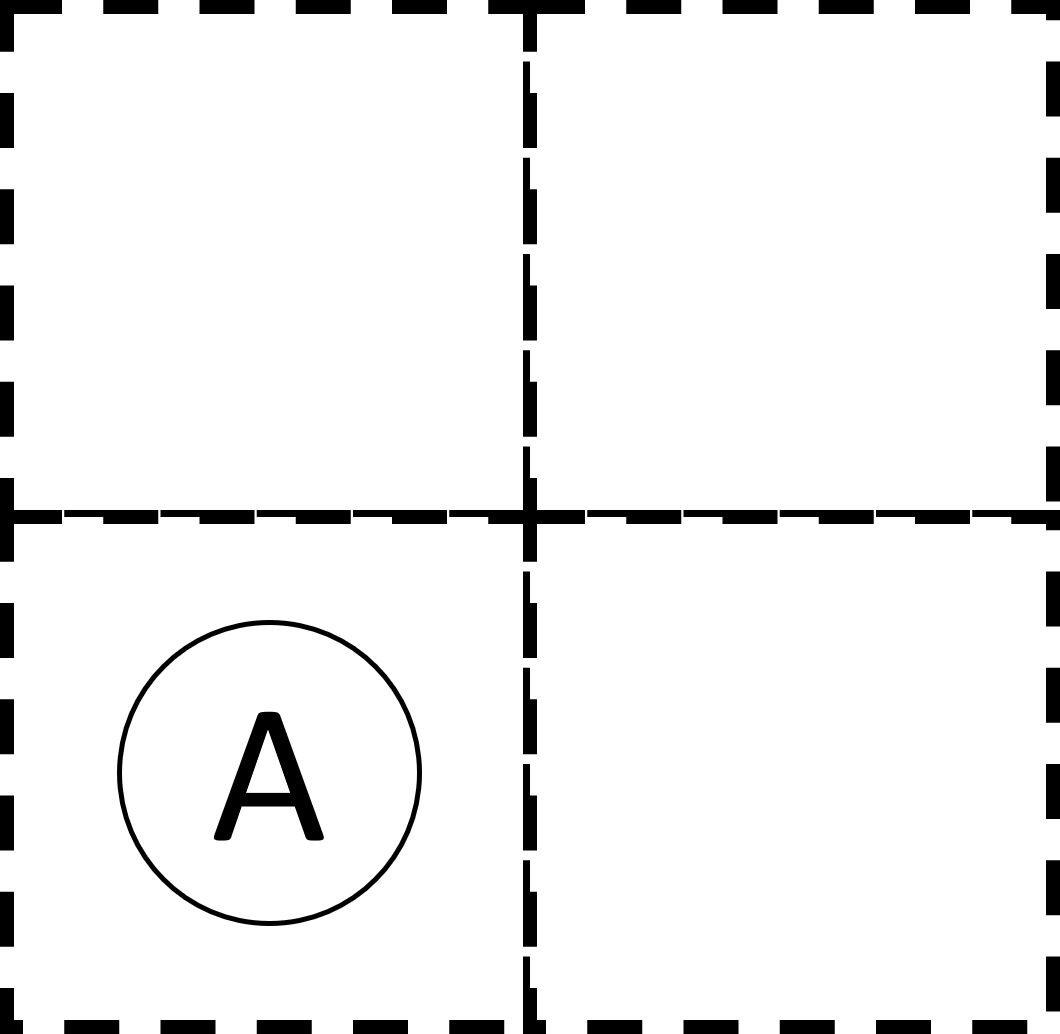
\includegraphics[width=0.5\linewidth]{2MathematicalFramework/InitialFramework/Images/2x2_no_walls_world_states/w2.png}
        \caption{$w_{2}$}
    \end{subfigure}
    \begin{subfigure}[b]{0.45\linewidth}
        \centering
        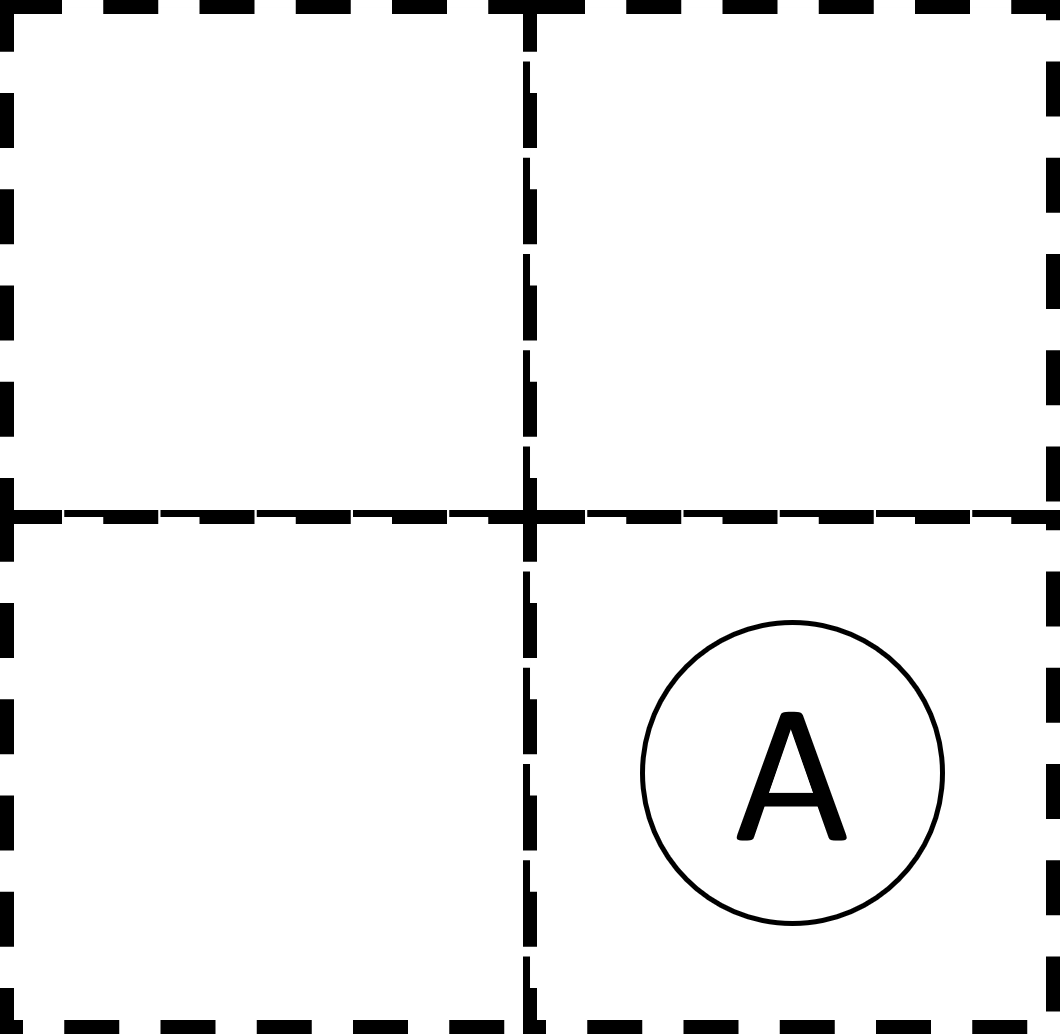
\includegraphics[width=0.5\linewidth]{2MathematicalFramework/InitialFramework/Images/2x2_no_walls_world_states/w3.png}
        \caption{$w_{3}$}
    \end{subfigure}
    \caption{The world states of a cyclical $2\times 2$ grid world $W_{c}$, where changes to the world are due to an agent moving either up, down, left, or right. The position of the agent in the world is represented by the position of the circled A.}
    \label{fig:2x2-cyclical-grid-world-states}
\end{figure}

We say the world being cyclical means that if the agent performs the same action enough times, then the agent will return to its starting position; for example, for the world $\mathscr{W}_{c}$ if the agent performs the action $U$ twice when the world is in state $w_{0}$ in Figure \ref{fig:2x2-cyclical-grid-world-states} then the world will transition into the state $w_{0}$ (i.e., $U^2 * w_{0} = w_0$).
The transition due to performing each action in each state can be found in Table \ref{tab:2x2-gridworld-minimum-transitions}.

\begin{table}
    \centering
    \begin{tabular}{c|c c c c c}
                &  $1$      & $U$       & $D$       & $L$       & $R$\\
         \hline
        $w_{0}$ & $w_{0}$   & $w_{2}$   & $w_{2}$   & $w_{1}$   & $w_{1}$\\
        $w_{1}$ & $w_{1}$   & $w_{3}$   & $w_{3}$   & $w_{0}$   & $w_{0}$\\
        $w_{2}$ & $w_{2}$   & $w_{0}$   & $w_{0}$   & $w_{3}$   & $w_{3}$\\
        $w_{3}$ & $w_{3}$   & $w_{1}$   & $w_{1}$   & $w_{2}$   & $w_{2}$\\
    \end{tabular}
    \caption{Each entry in this table shows the outcome state of the agent performing the action given in the column label when in the world state given by the row label.}
    \label{tab:2x2-gridworld-minimum-transitions}
\end{table}

The transitions shown in Table \ref{tab:2x2-gridworld-minimum-transitions} can be represented as the transition diagram given in Figure \ref{fig:2x2-cyclical-min-trans}.
It should be noted that, since the structure of the diagram is wholly dependent on the arrows between the world states, the positioning of the world states is an arbitrary choice.

\begin{figure}
    \centering
    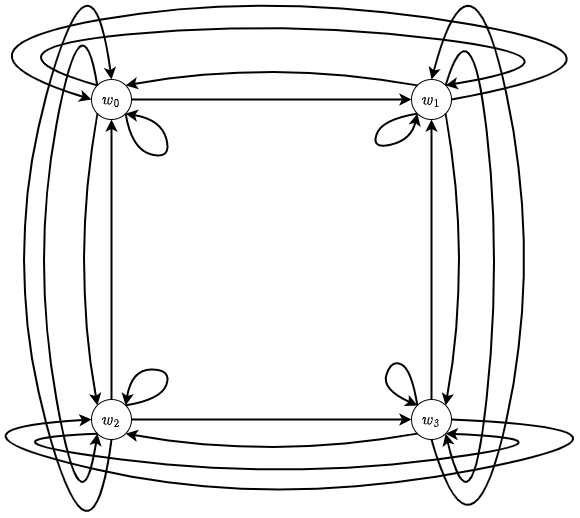
\includegraphics[width=0.5\linewidth]{2MathematicalFramework/InitialFramework/Images/2x2-cyclical-min-trans.drawio.png}
    \caption{A transition diagram for the transitions shown in Table \ref{tab:2x2-gridworld-minimum-transitions}.}
    \label{fig:2x2-cyclical-min-trans}
\end{figure}

%%%%%%%%%%%%%%%%%%%%%%%%%%%%%%%%%%%%%%%%%%%%%%%
\subsection{\sout{Agents}}
\sout{We now define the actions of agents as collections of transitions that are labelled by their associated action.
We then define some relevant properties of these actions.}

%%%%%%%%%%%%%%%%%%%%%%%%%%%%%%%%%%%%%%%%%%%%%%%
\textbf{\sout{Actions of an agent as labelled transitions}}\label{sec:Agent actions as labelled transitions}

\sout{Consider a set $\hat{A}$ called the set of \textit{minimum actions}.
Let the set $A$ be the set of all finite \whendraft{\textbf{and infinite}} sequences formed from the elements of the set $\hat{A}$; we call $A$ the set of \textit{actions}.}

\sout{Consider a set $\hat{D}_{A} \subset D$, where $1_{w} \in \hat{D}_{A}$ for all $w \in W$; we call $\hat{D}_{A}$ the set of \textit{minimum action transitions}.
We consider a labelling map $\hat{l}: \hat{D}_{A} \to \hat{A}$ such that:}

\begin{enumerate}
    \item \sout{Any two distinct transitions leaving the same world state are labelled with different actions.}
    \begin{action_condition}
        \sout{For any $d,d' \in \hat{D}_{A}$ with $s(d)=s(d')$, $\hat{l}(d) \neq \hat{l}(d')$.}
    \end{action_condition}

    \item There is an identity action that leaves any world state unchanged.
    \begin{action_condition}
        There exists an action $1 \in \hat{A}$ such that $\hat{l}(1_{w})=1$ for all $w \in W$.
        We call $1$ the \textit{identity action}.
    \end{action_condition}
    
\end{enumerate}

\sout{Figure ref[fig:l-map-for-transitions-from-and-to-w0] demonstrates how the map $l$ maps transitions in $D$ to the elements in $A$ for the transitions shown in Figure \ref{fig:2x2-cyclical-min-actions-standard}.}

\whendraft{
\begin{remark}
    \hyperref[actcon:action-gives-single-outcome]{Action condition \ref*{actcon:action-gives-single-outcome}} means that for each $w \in W$, there is a subset of $\hat{D}_{A}$ given by $\{d \mid d \in \hat{D}_{A}\textit{, } s(d)=w\}$; for each of these subsets, the elements of the subset are uniquely labelled (within the subset) by $l$.
    In other words, the transitions in $D_{A}$ with source $s(d)$ are uniquely labelled by $\hat{l}$ for all $d \in D_{A}$.
\end{remark}
}


\sout{
Given $\hat{D}_{A}$ as defined above and satisfying  action condition \ref{actcon:action-gives-single-outcome} and  action condition \ref{actcon:identity-action}, we define $Q_{D_{A}} = (W, \hat{D}_{A}, s_{A}, t_{A})$, where $s_{A}, t_{A}$ are the restrictions of $s,t$ to the set $\hat{D}_{A}$.
We now define a set $D_{A}$, the set of \textit{action transitions}, which is the set of all paths of $Q_{D_{A}}$.
We extend the map $\hat{l}$ to a map $l: D_{A} \to A$ such that if $d = \hat{d}_{n} \circ ... \circ \hat{d}_{1}$ then $l(d) = \hat{l}(\hat{d}_{n}) ... \hat{l}(\hat{d}_{1})$.

For $d \in D_{A}$ with $s(d) = w$, $t(d) = w'$ and $l(d) = a$, we will often denote $d$ by $d: w \xrightarrow{a} w'$.

If an action $a \in A$ is expressed in terms of its minimum actions as $a = \hat{a}_{n} \circ ... \circ \hat{a}_{1}$, then $a = l(d) = l(\hat{d}_{n} \circ ... \circ \hat{d}_{1}) = \hat{l}(\hat{d}_{n}) \circ ... \circ \hat{l}(\hat{d}_{1}) = \hat{a}_{n} \circ ... \circ \hat{a}_{1}$, where the $\hat{a}_{i}$ are called \textit{minimum actions}.
}


\begin{remark}
    \textbf{Kill this ?}
    For a given $w \in W$, we can label transitions in $D_{A}$ with an appropriate element of $A$ through the following: for each $d \in D_{A}$ with $s(d)=w$, express $d$ in terms of its minimum transitions in $D_{A}$ as $d = d_{n} \circ ... \circ d_{2} \circ d_{1}$; if $\hat{l}(d_{i}) = a_{i}$ then $d$ is labelled with $a_{n}...a_{2}a_{1} \in A$.
    We denote the map that performs this labelling by $l: D_{A} \to A$.
\end{remark}

Figure \ref{fig:2x2-cyclical-min-actions-standard} shows how transitions are labelled with actions in our $2 \times 2$ cyclical world example.
We only show the minimum actions for simplicity but there are actually infinite action transitions between each pair of world states; for example, the action transitions from $w_{0}$ to $w_{1}$ include those labelled by: $D \circ R$, $D \circ R \circ 1^{n}$ ($n \in \mathbb{N}$), $1^{n} \circ D \circ R$ ($n \in \mathbb{N}$), $D \circ R \circ (L \circ R)^{n}$ ($n \in \mathbb{N}$) etc...

\begin{figure}
    \centering
    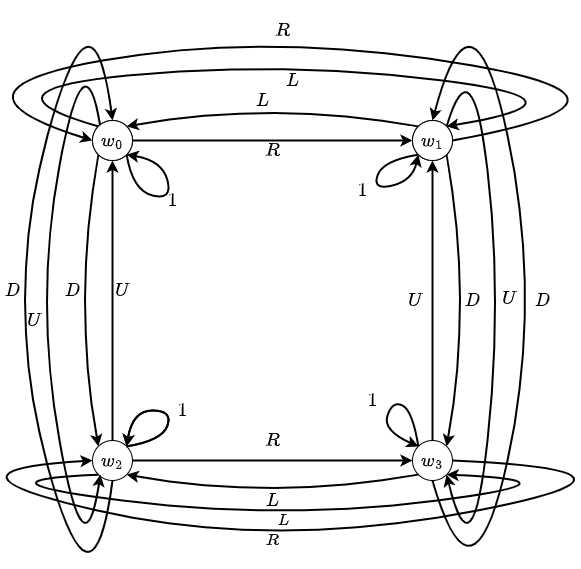
\includegraphics[width=0.5\linewidth]{2MathematicalFramework/InitialFramework/Images/2x2-cyclical-min-actions.drawio.png}
    \caption{Labelling the transitions in Figure \ref{fig:2x2-cyclical-min-trans} with the relevant actions in $A$.}
    \label{fig:2x2-cyclical-min-actions-standard}
\end{figure}

\paragraph{\sout{Effect of actions on world states}}
\sout{
We define the effect of the action $a \in A$ on world state $w \in W$ as the following: if there exists $d \in D_{A}$ such that $s(d)=w$ and $l(d)=a$, then $a * w = t(d)$; if there does not exist $d \in D_{A}$ such that $s(d)=w$ and $l(d)=a$, then we say that $a * w$ is \textit{undefined}.
The effect of actions on world states is well-defined due to action condition \ref{actcon:action-gives-single-outcome}.
}
\sout{
We can apply the minimum actions that make up an action to world states individually: if $a * w$ is defined and $a = \hat{a}_{k}...\hat{a}_{1}$ then $a * w = (\hat{a}_{k}...\hat{a}_{1}) * w = \hat{a}_{k}...\hat{a}_{2} * (\hat{a}_{1} * w)$.
}

\sout{
Physically, the identity action $1 \in A$ corresponds to the no-op action (\textit{i.e.}, the world state does not change due to this action).
}

\paragraph{\sout{Actions as (partial) functions}}
\sout{
Consider all the transitions that are labelled by a particular action $a \in A$.
Together these transitions form a partial function $f_{a}: W \to W$ because for any $w \in W$ either $a * w$ is undefined or $a * w$ is defined and there is a unique world state $w' \in W$ for which $a * w = w'$ (due to condition 1).
}

\sout{
$f_{a}$ is not generally surjective because for a given $w \in W$ there is not necessarily a transition $d \in D$ with $l(d) = a$ and $t(d) = w$.
}

\sout{
$f_{a}$ is not generally injective because it is possible to have an environment where $f_{a}(w)=f_{a}(w')$ for some $w \in W$ different from $w' \in W$.
}

\sout{
We can also reproduce these functions using the formalism given by \autocite{caselles2019symmetry}, which describes the dynamics of the world in terms of a multivariate function $f: A \times W \to W$.
If we let $f: A \times W \to W$ be the dynamics of the environment then the transition caused by an action $a \in A$ on a world state $w \in W$ (where $a * w$ is defined) is given by $(a,w) \mapsto f(a,w) = a * w$.
}

\sout{
Mathematically, we curry the function $f: A \times W \to W$ to give a collection $\{f_{a}\}$ of partial functions with a partial function $\hat{f}(a)=f_{a}: W \to W$ for each action $a \in A$ as $\textit{Curry}: (f: A \times W \to W) \to (f_{a}: W \to W)$.
}